\documentclass[12pt, a4paper]{article}

\title{\textsc{Computer Architecture} Homework 6}
\author{110062219}
\date{\today}

\usepackage{amsmath}
\usepackage{amssymb}
\usepackage{caption}
\usepackage{subcaption}
\usepackage{tikz}
\usepackage{pgfplots}
\usepackage{listings}
\usepackage{float}
\usepackage{tabularx}
\usepackage{makecell}
\usepackage{hyperref}
%\usepackage{geometry}[margin=2cm]

\lstset{
  breaklines=true,
  basicstyle=\ttfamily,
}

\definecolor{nthu}{HTML}{7F1084}

% \renewcommand{\ttdefault}{pcr}

\begin{document}

\maketitle
\tableofcontents

\section{Cache Cases}

Since there is no any instruction write to memory in my assembly codes of prior assignment, I did the experiments on the provided \texttt{KMP.elf}.

\subsection{Cache Insertion}

\begin{figure}[htbp]
\begin{subfigure}{\linewidth}
\centering
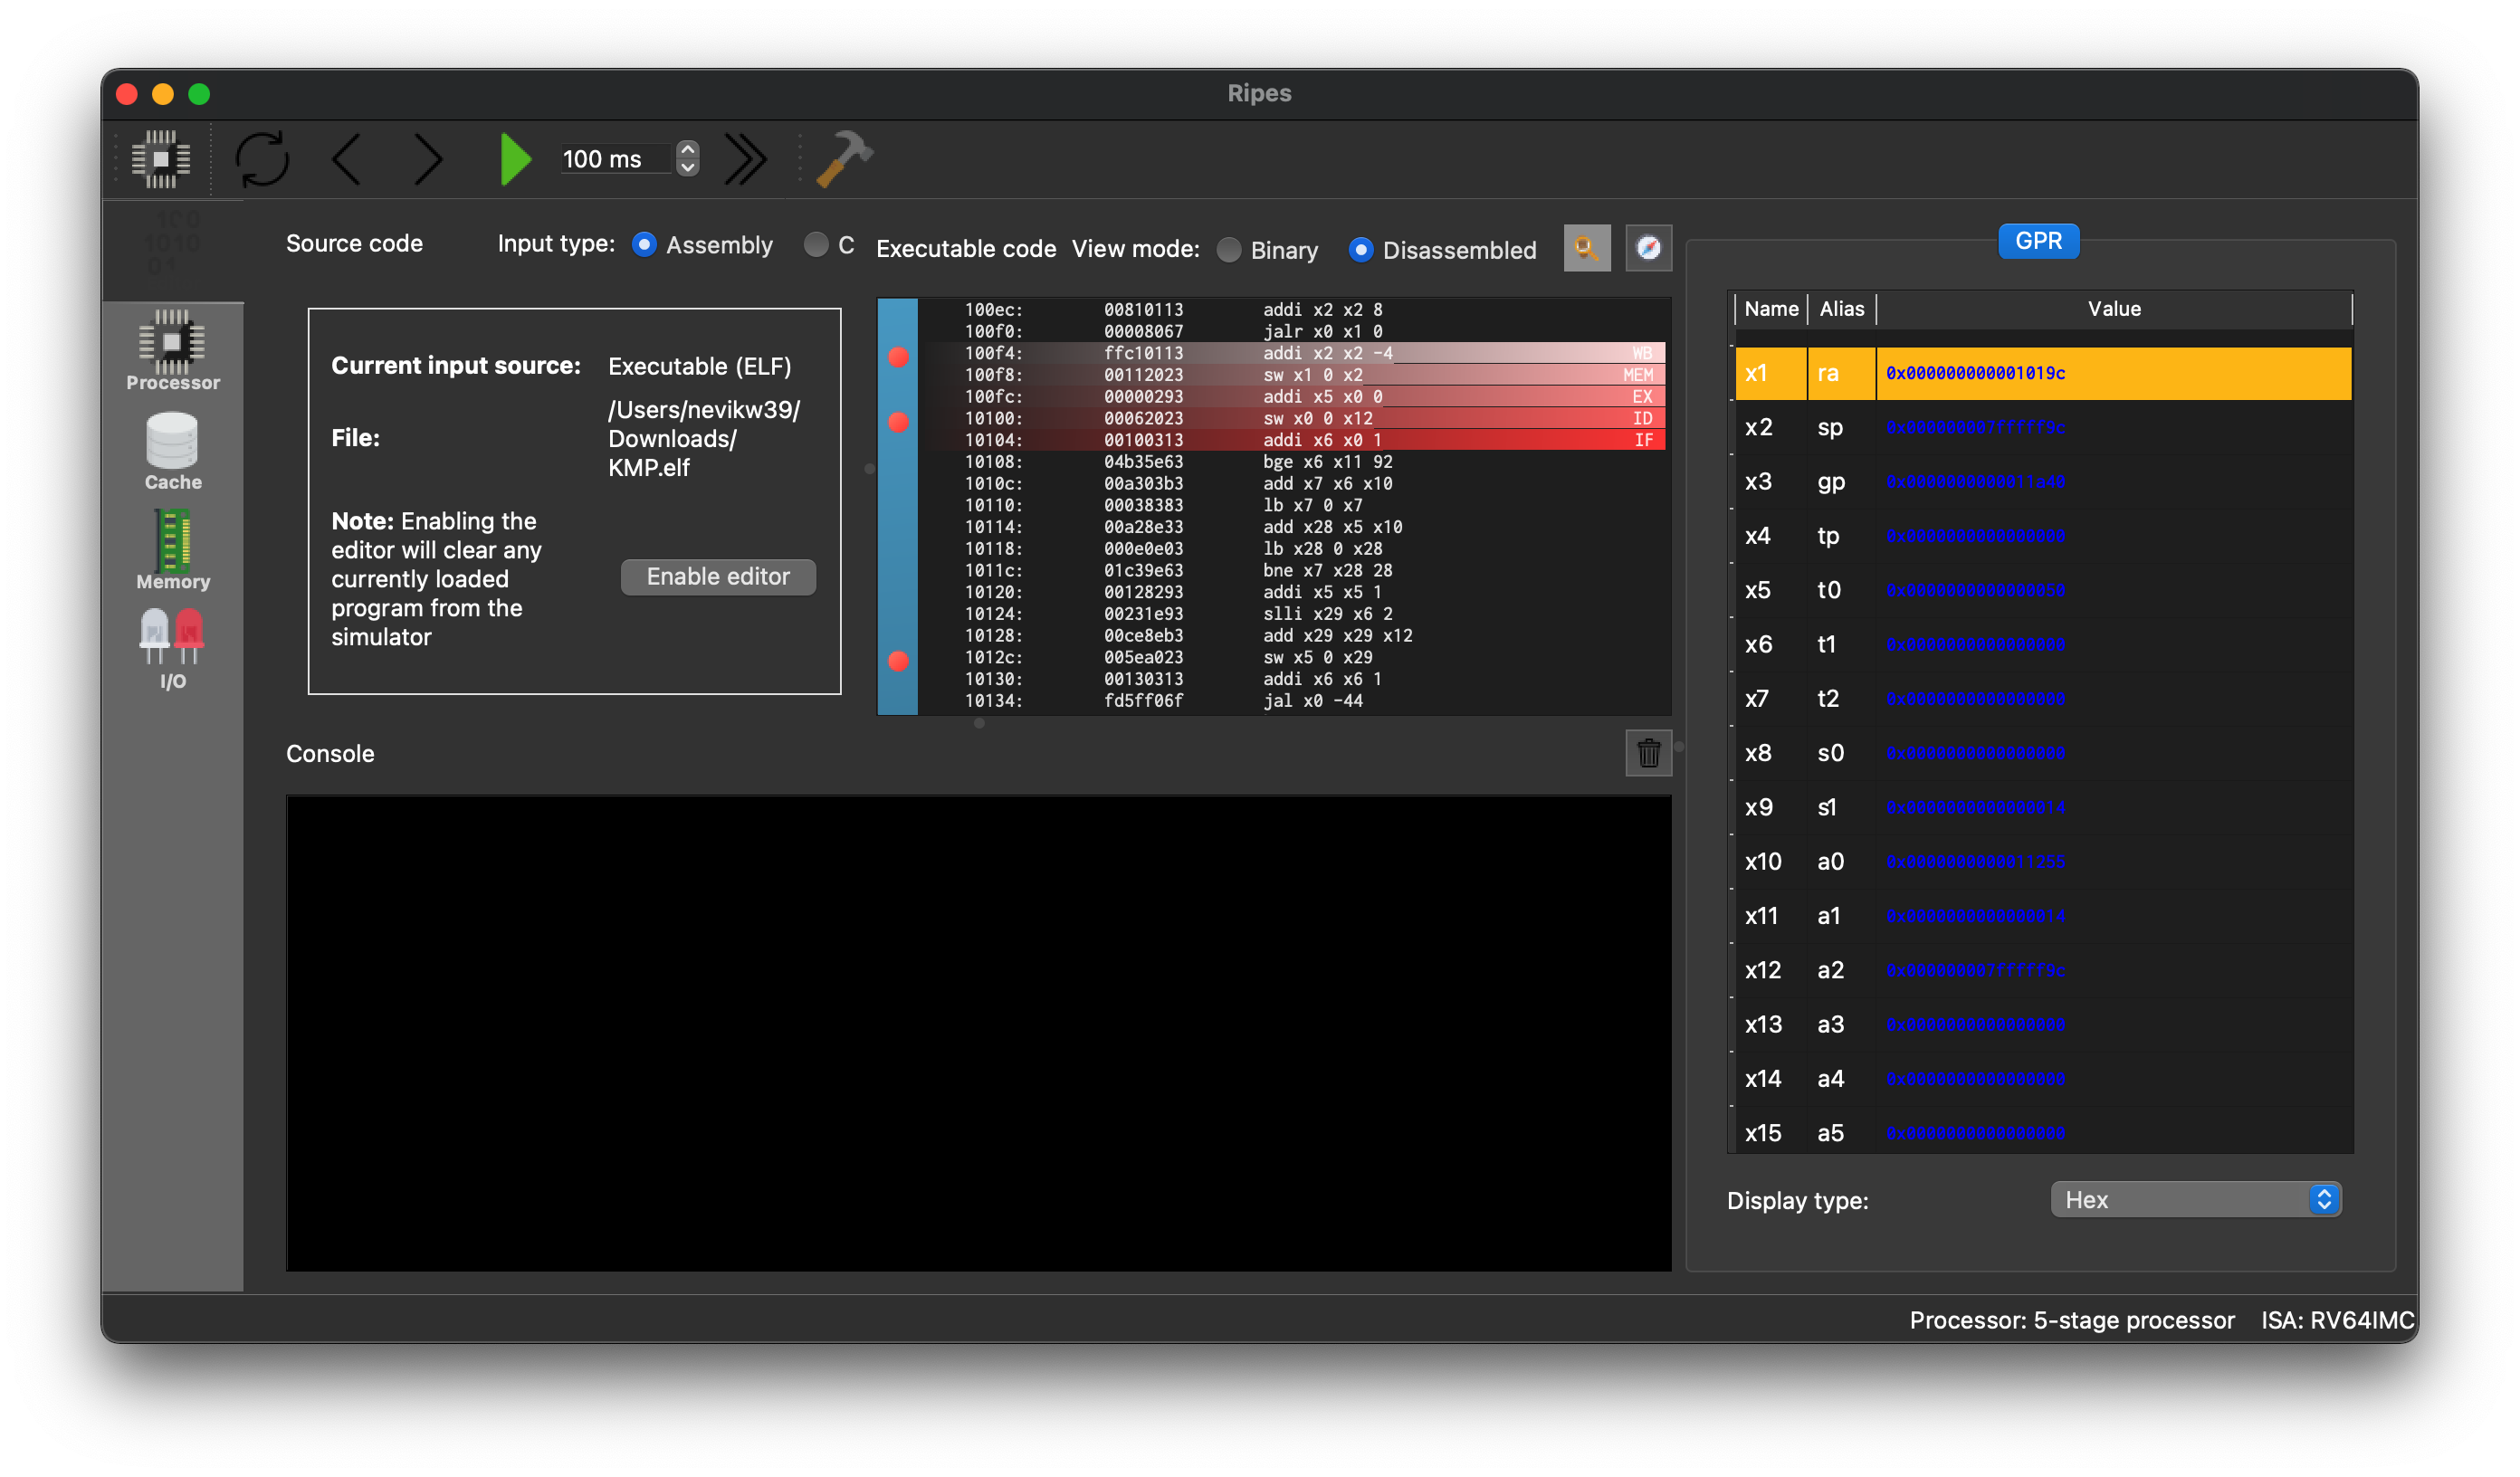
\includegraphics[width=.69\linewidth]{a}
\caption{The instruction}
\end{subfigure}
\begin{subfigure}{\linewidth}
\centering
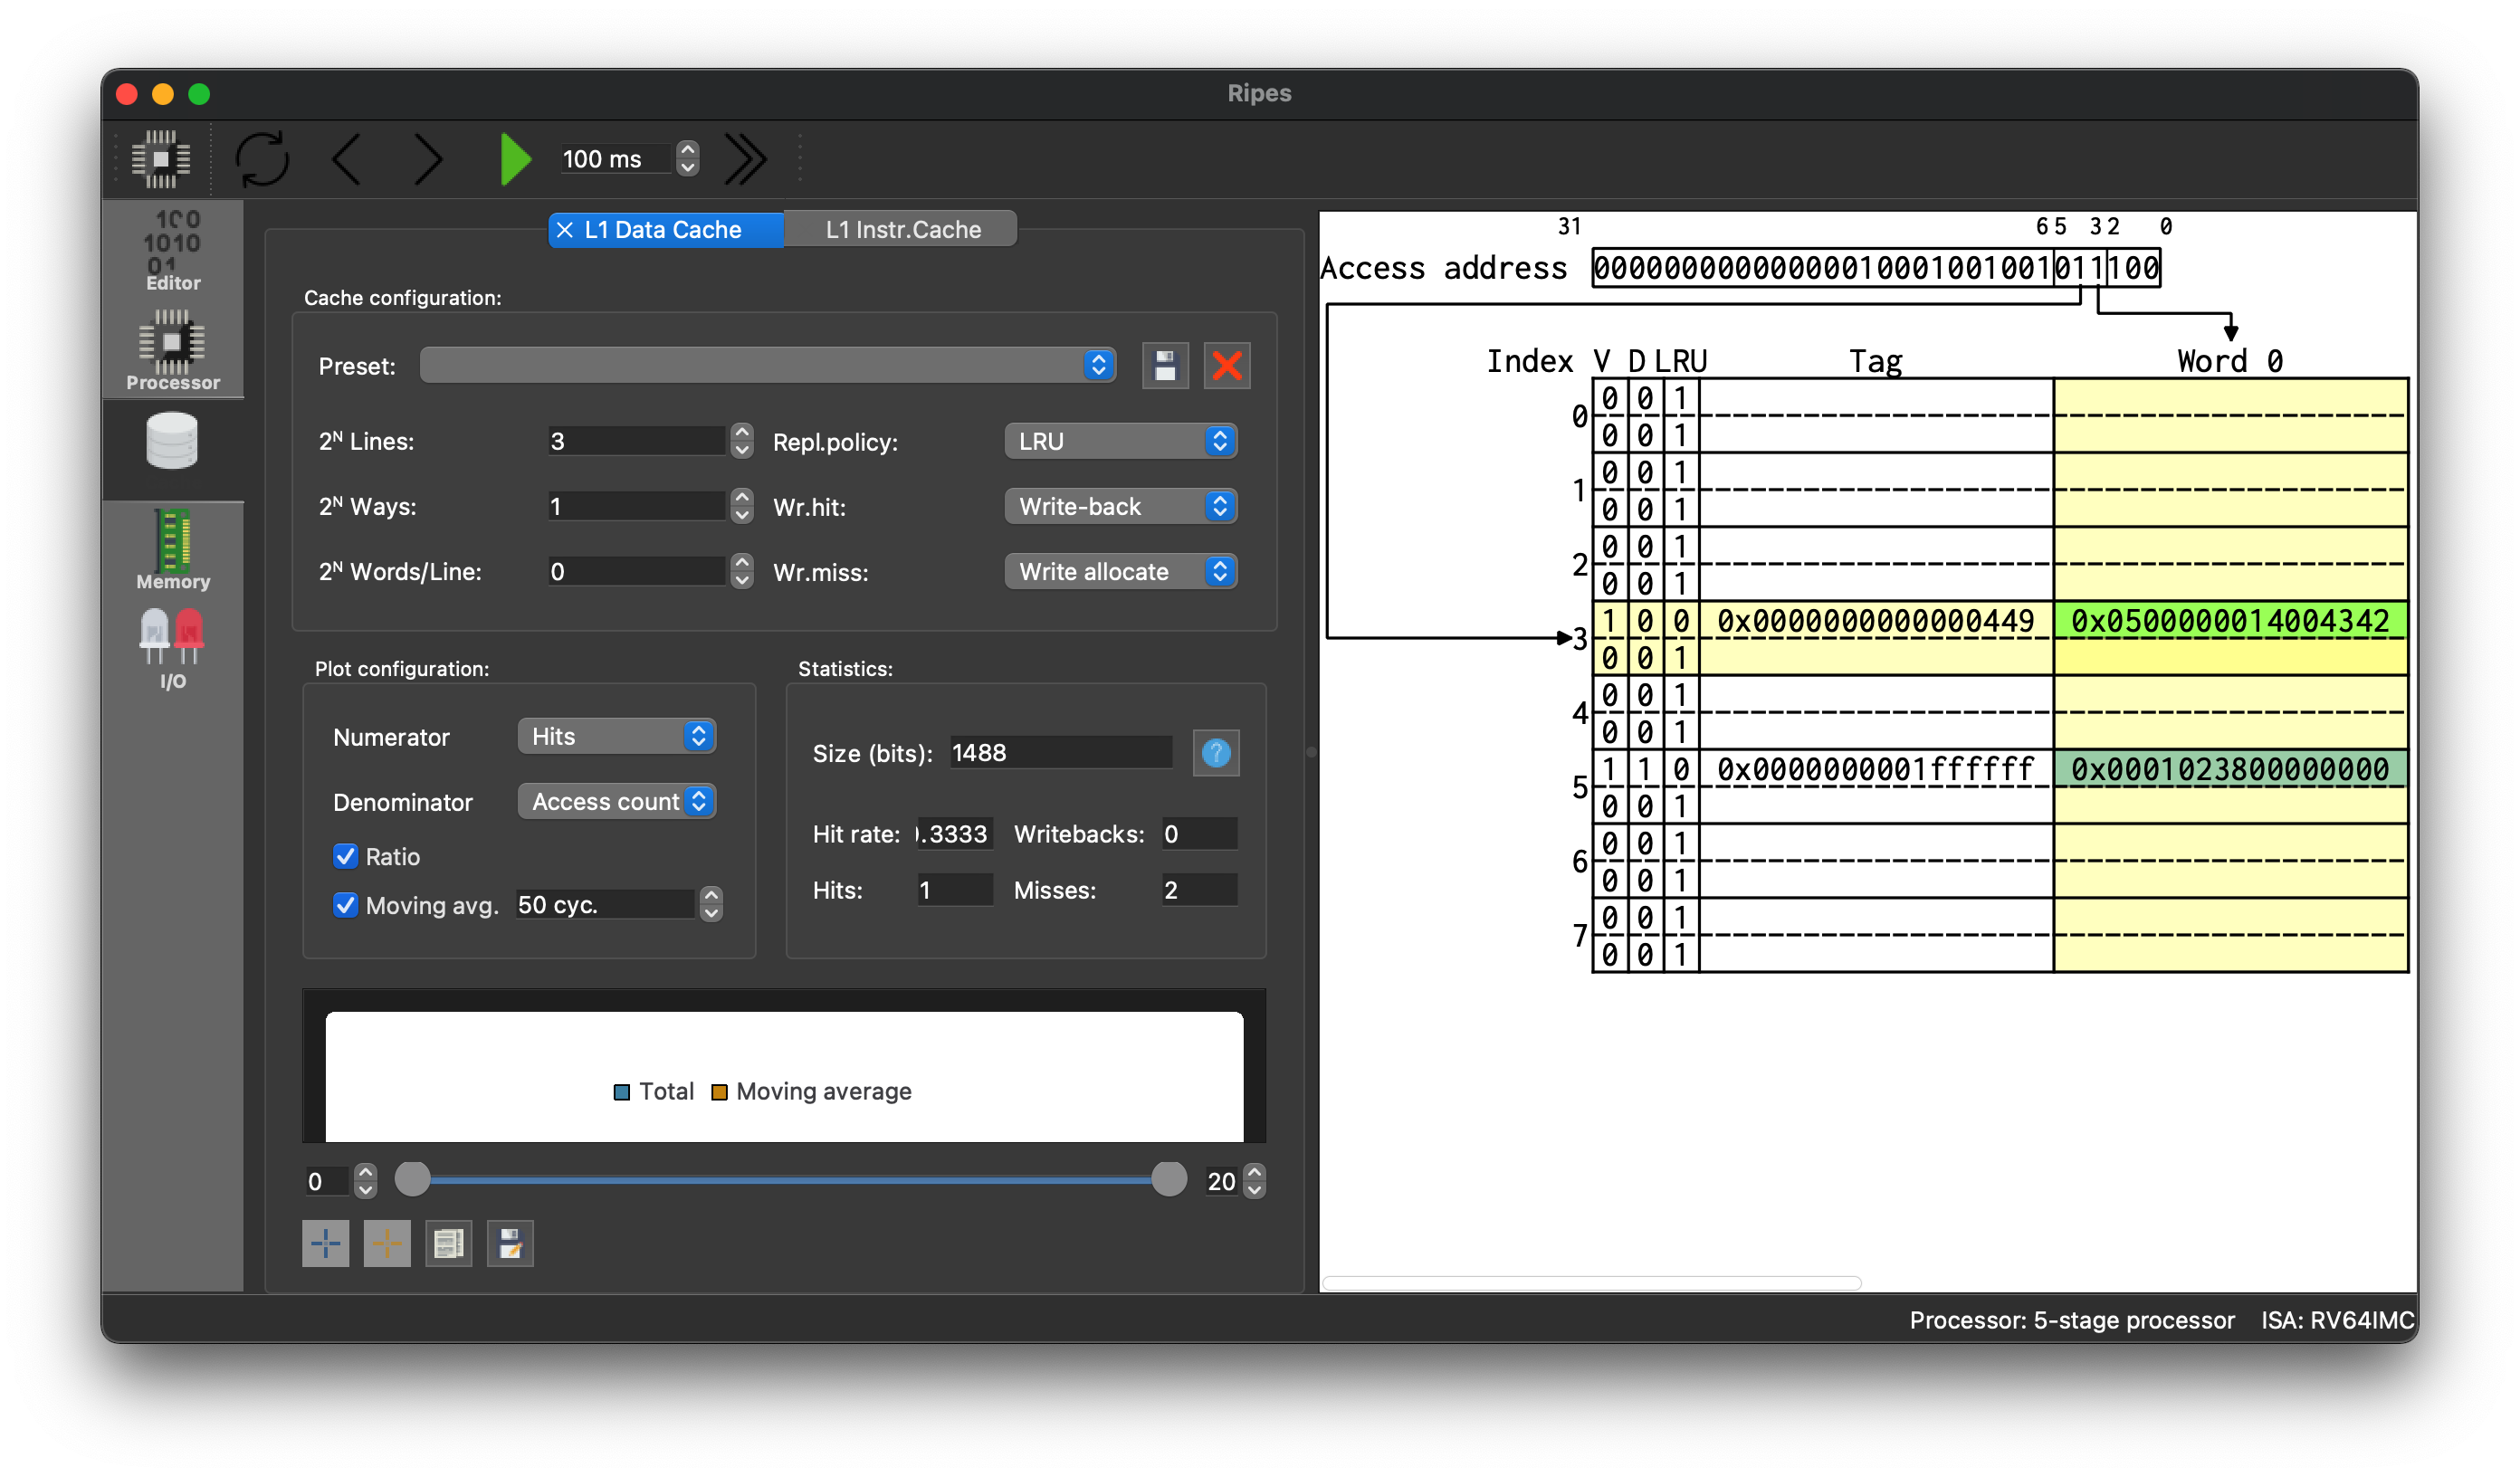
\includegraphics[width=.807\linewidth]{a0}
\caption{Before}
\label{fig:1a0}
\end{subfigure}
\begin{subfigure}{\linewidth}
\centering
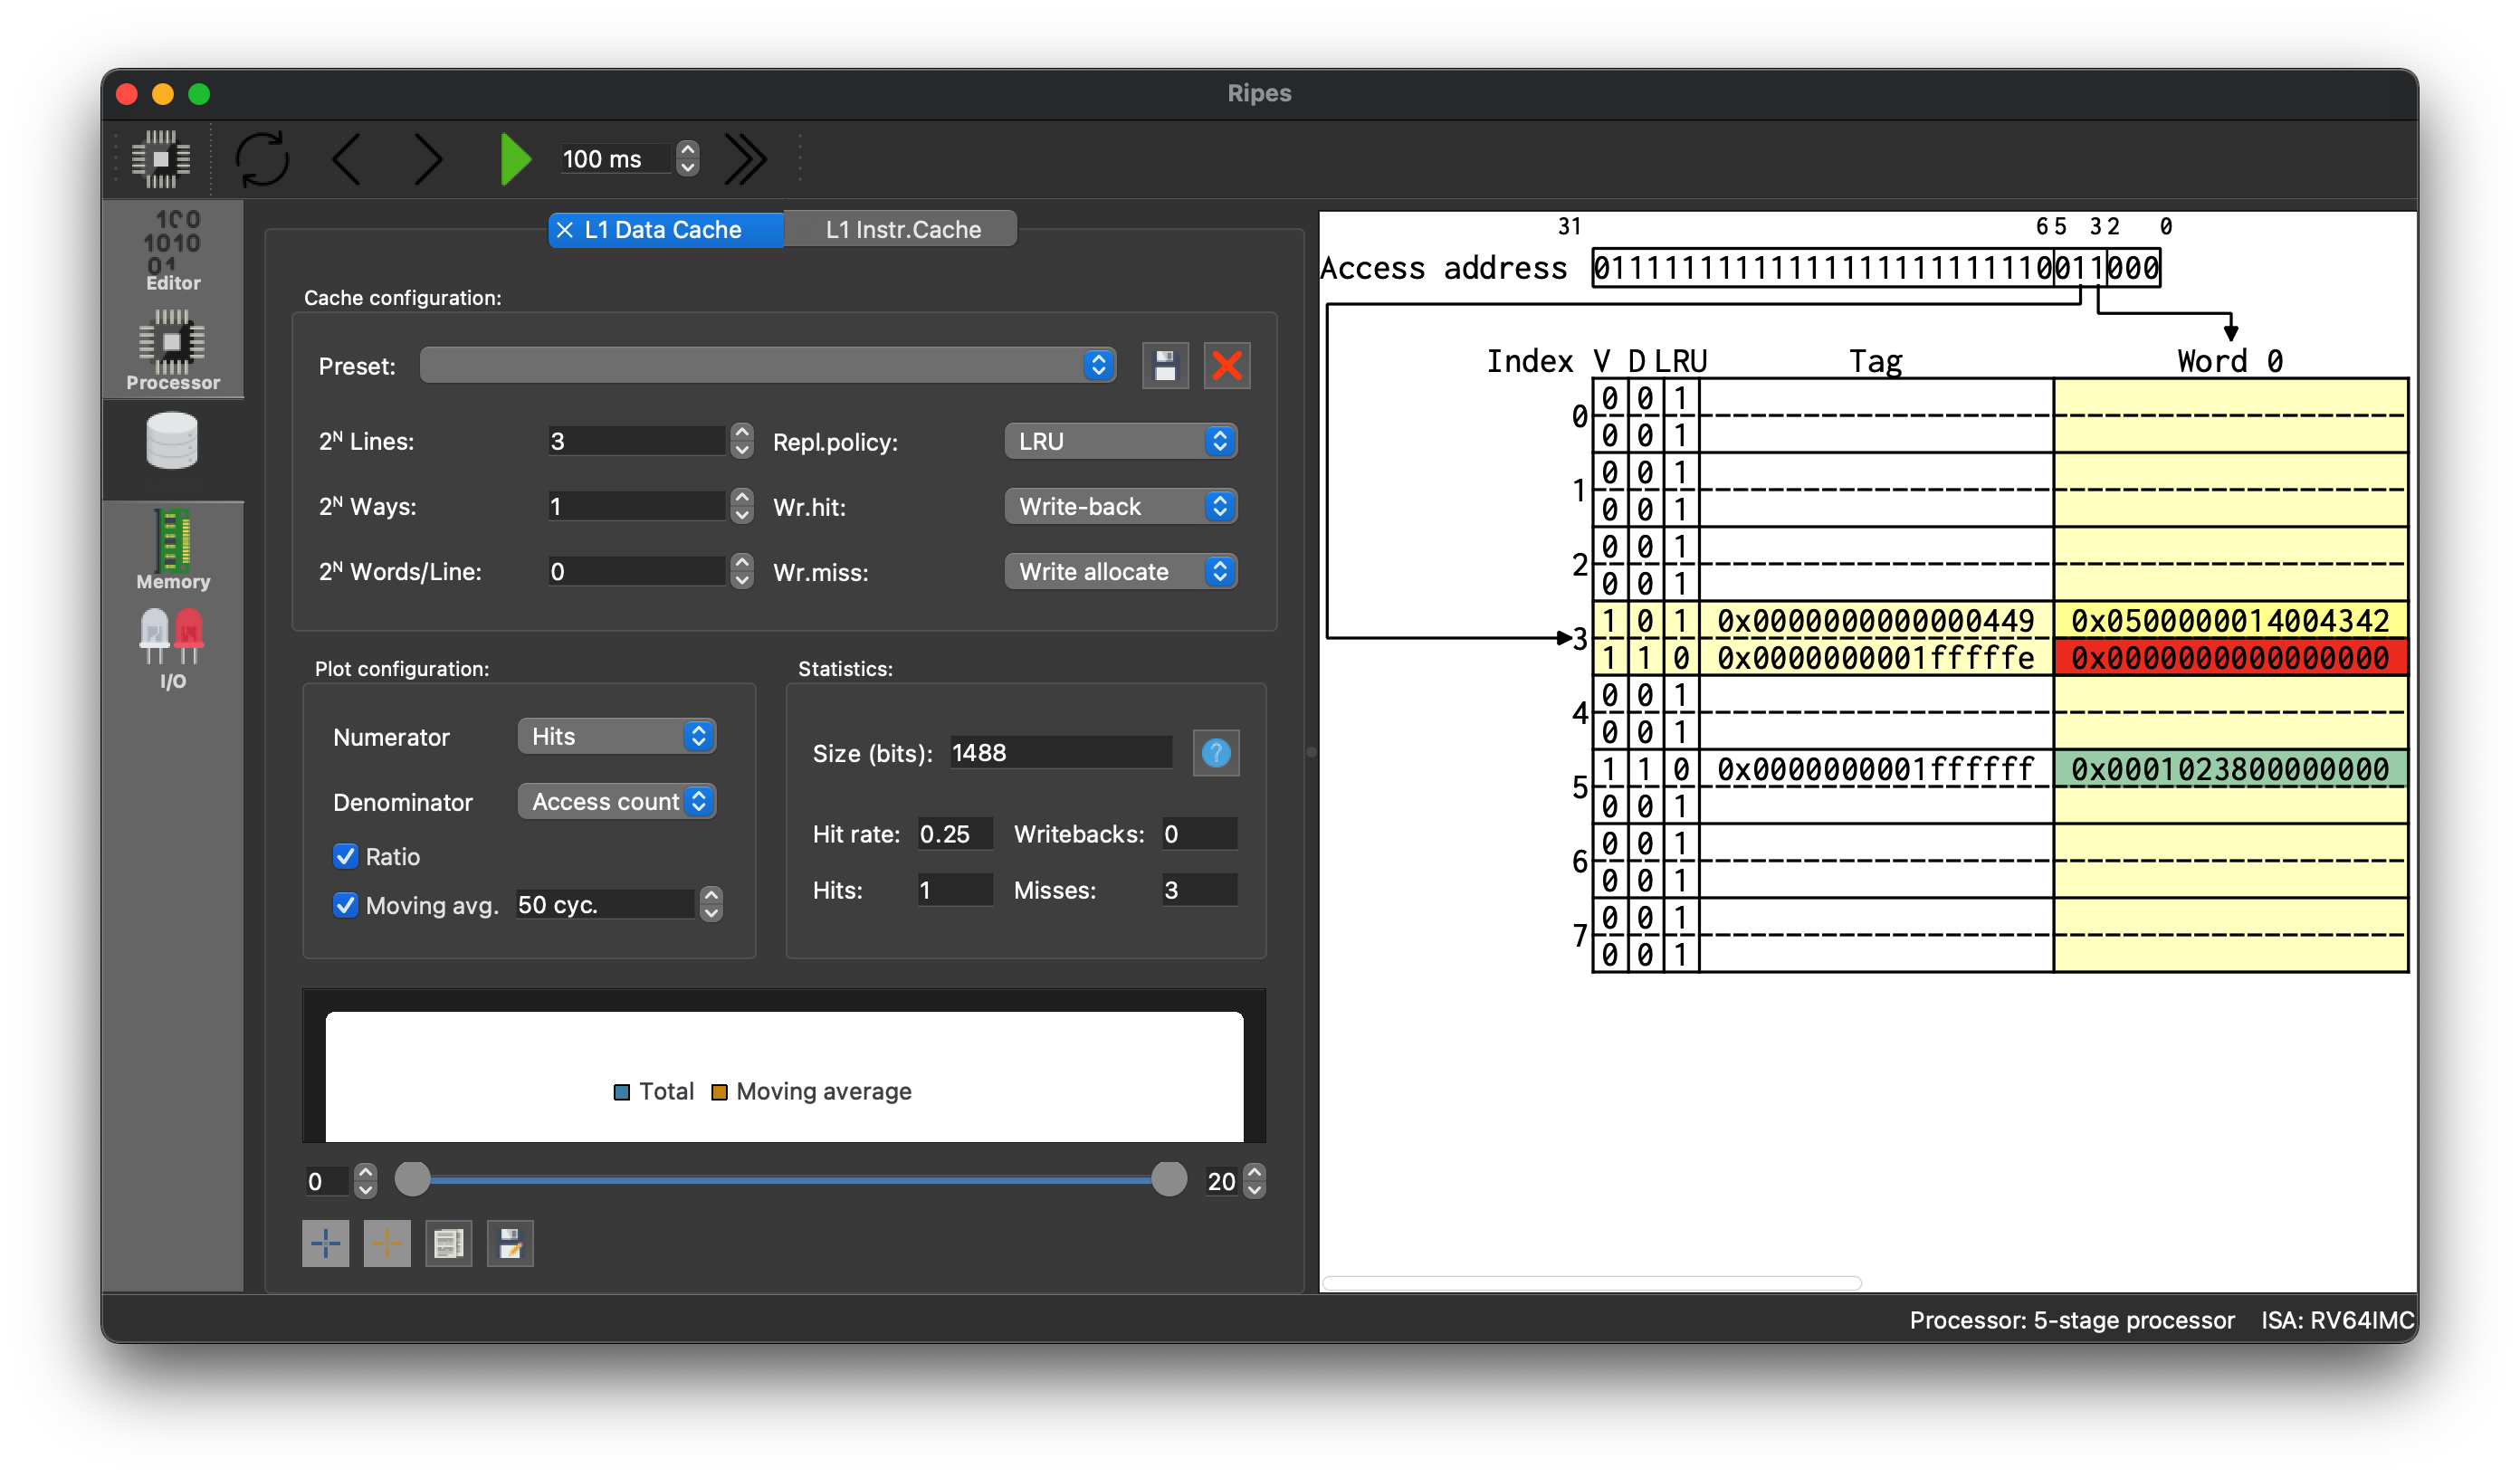
\includegraphics[width=.807\linewidth]{a1}
\caption{After}
\label{fig:1a1}
\end{subfigure}
\caption{Cache Insertion}
\label{fig:1a}
\end{figure}

The screenshots are in Figure \ref{fig:1a}. Before the \texttt{sw} instruction, the set of index 3 contained exact 1 valid way whose LRU bit is 0. After that instruction, the LRU bit of the original way becomes 1 and the one of the newly-allocated way is 0.

\subsection{Write Hit}

\begin{figure}[htbp]
\begin{subfigure}{\linewidth}
\centering
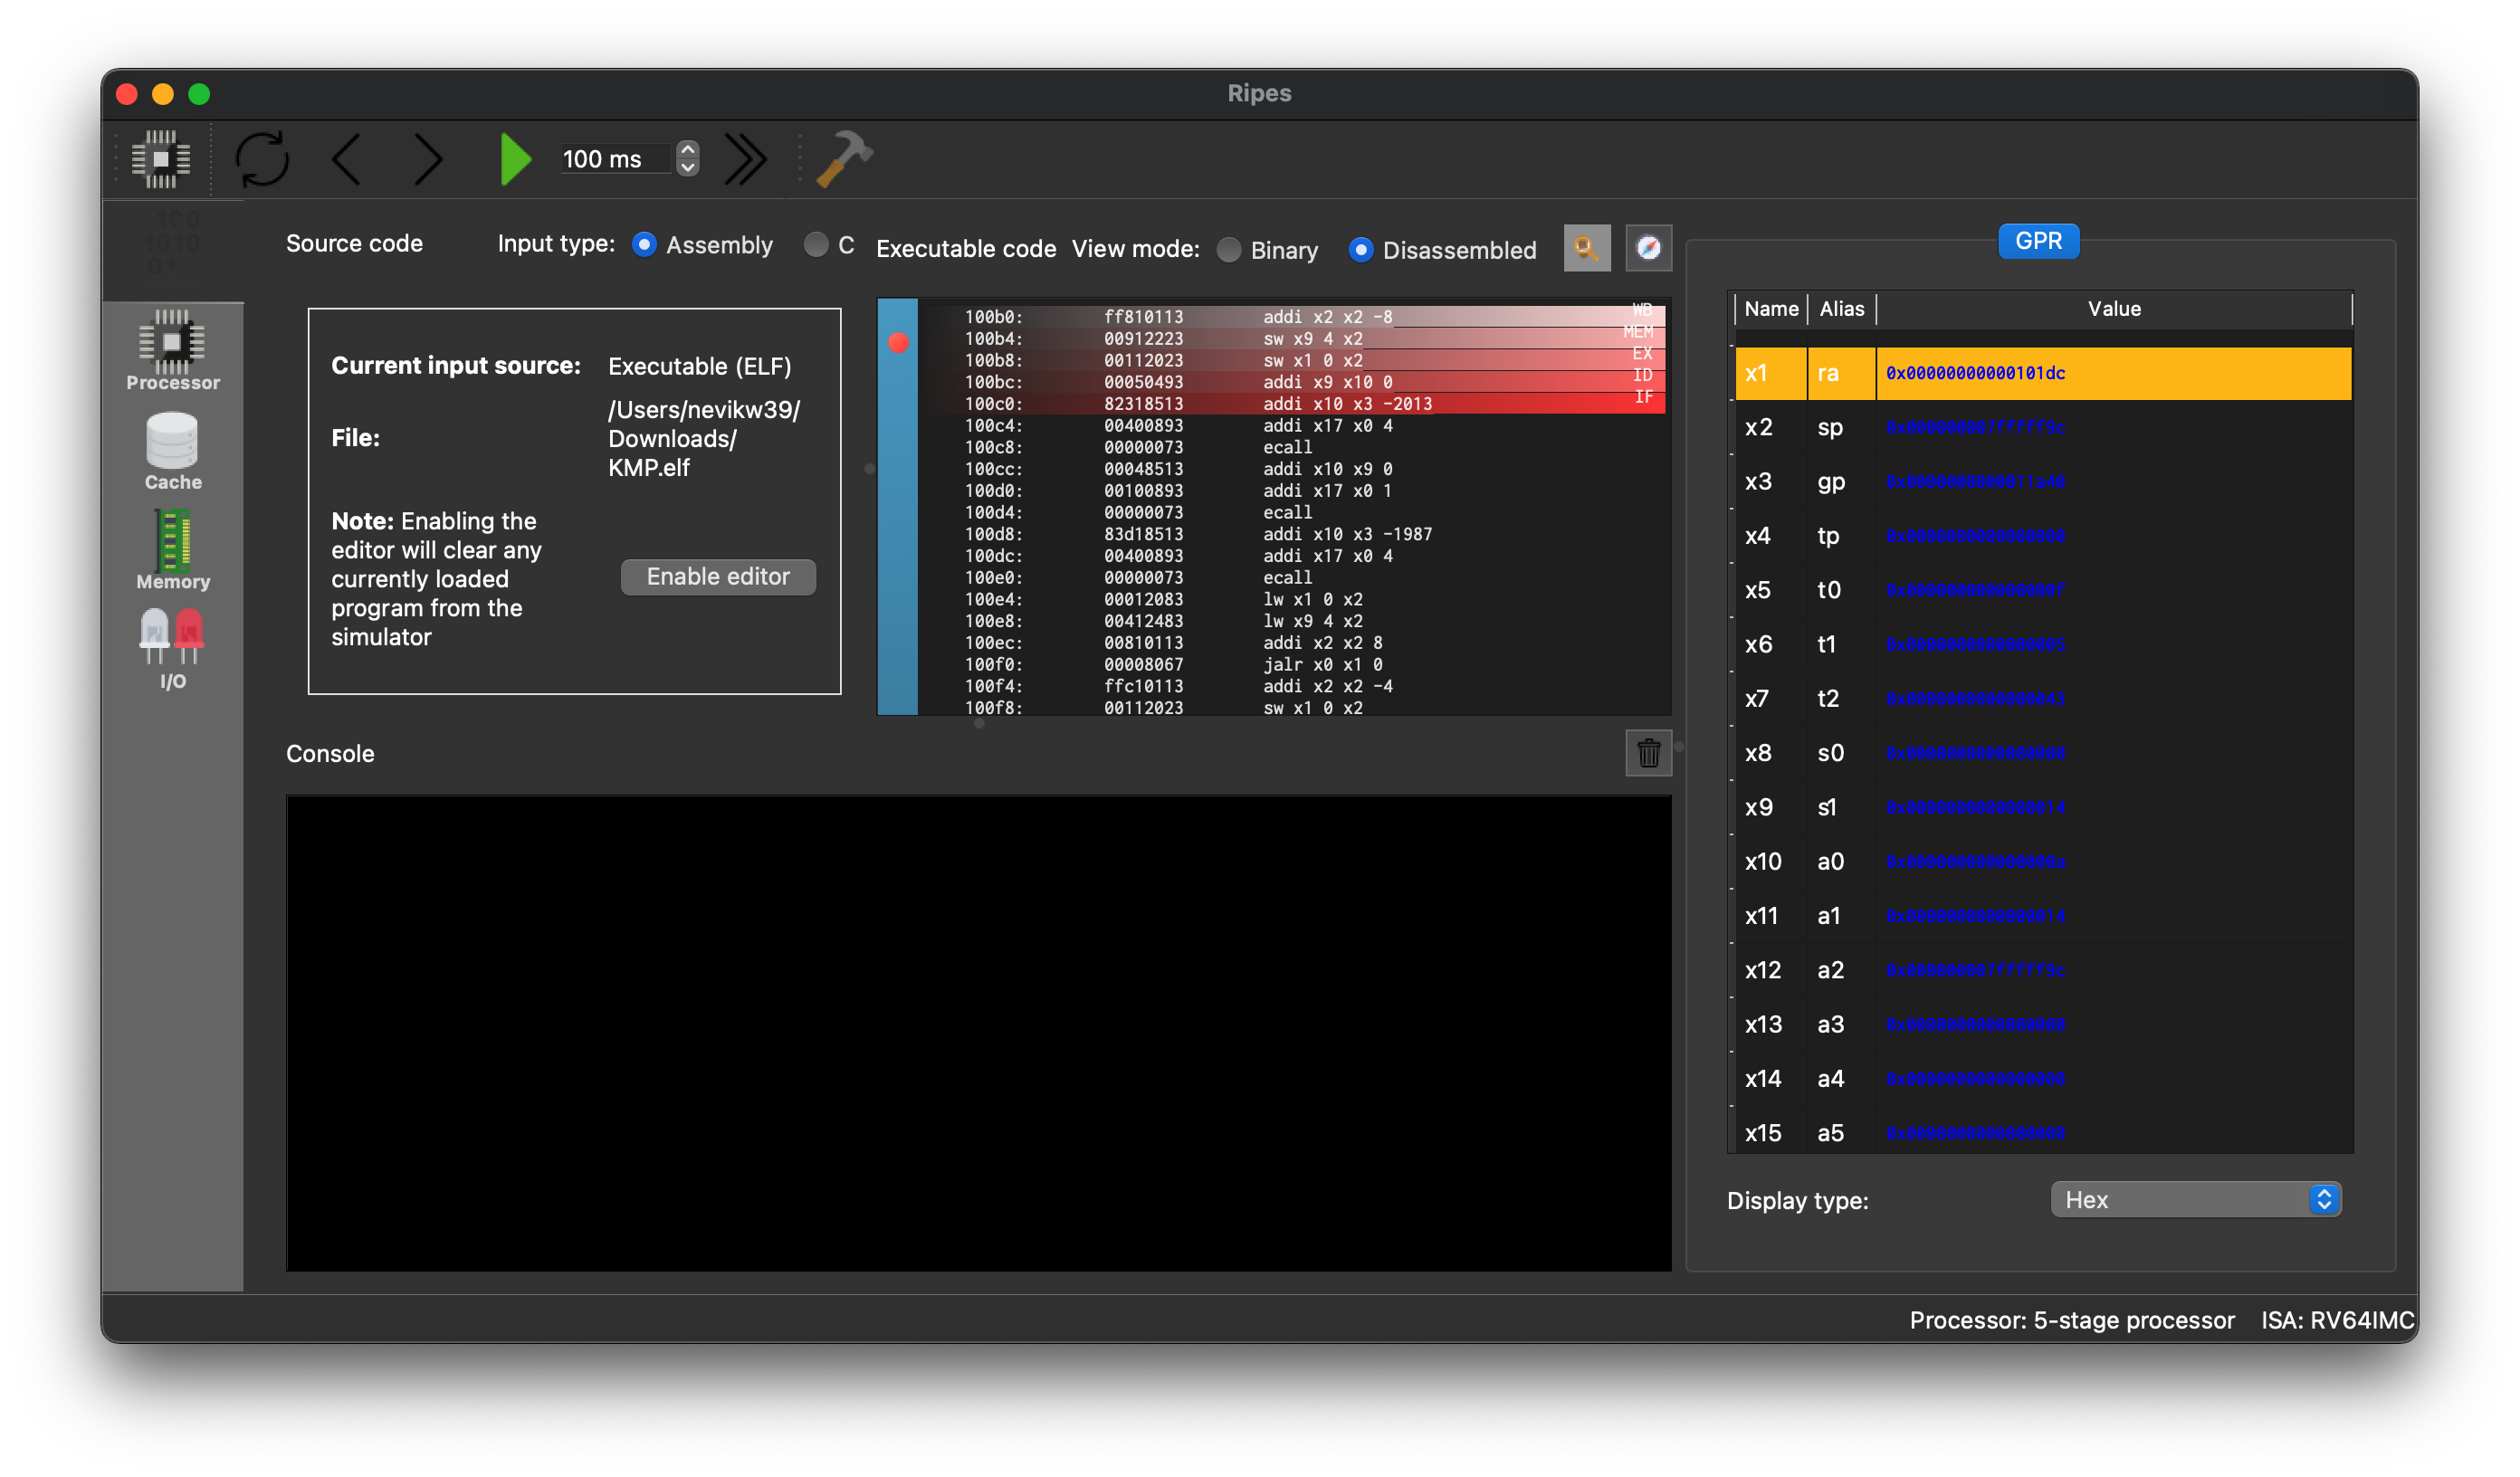
\includegraphics[width=.69\linewidth]{b}
\caption{The instruction}
\end{subfigure}
\begin{subfigure}{\linewidth}
\centering
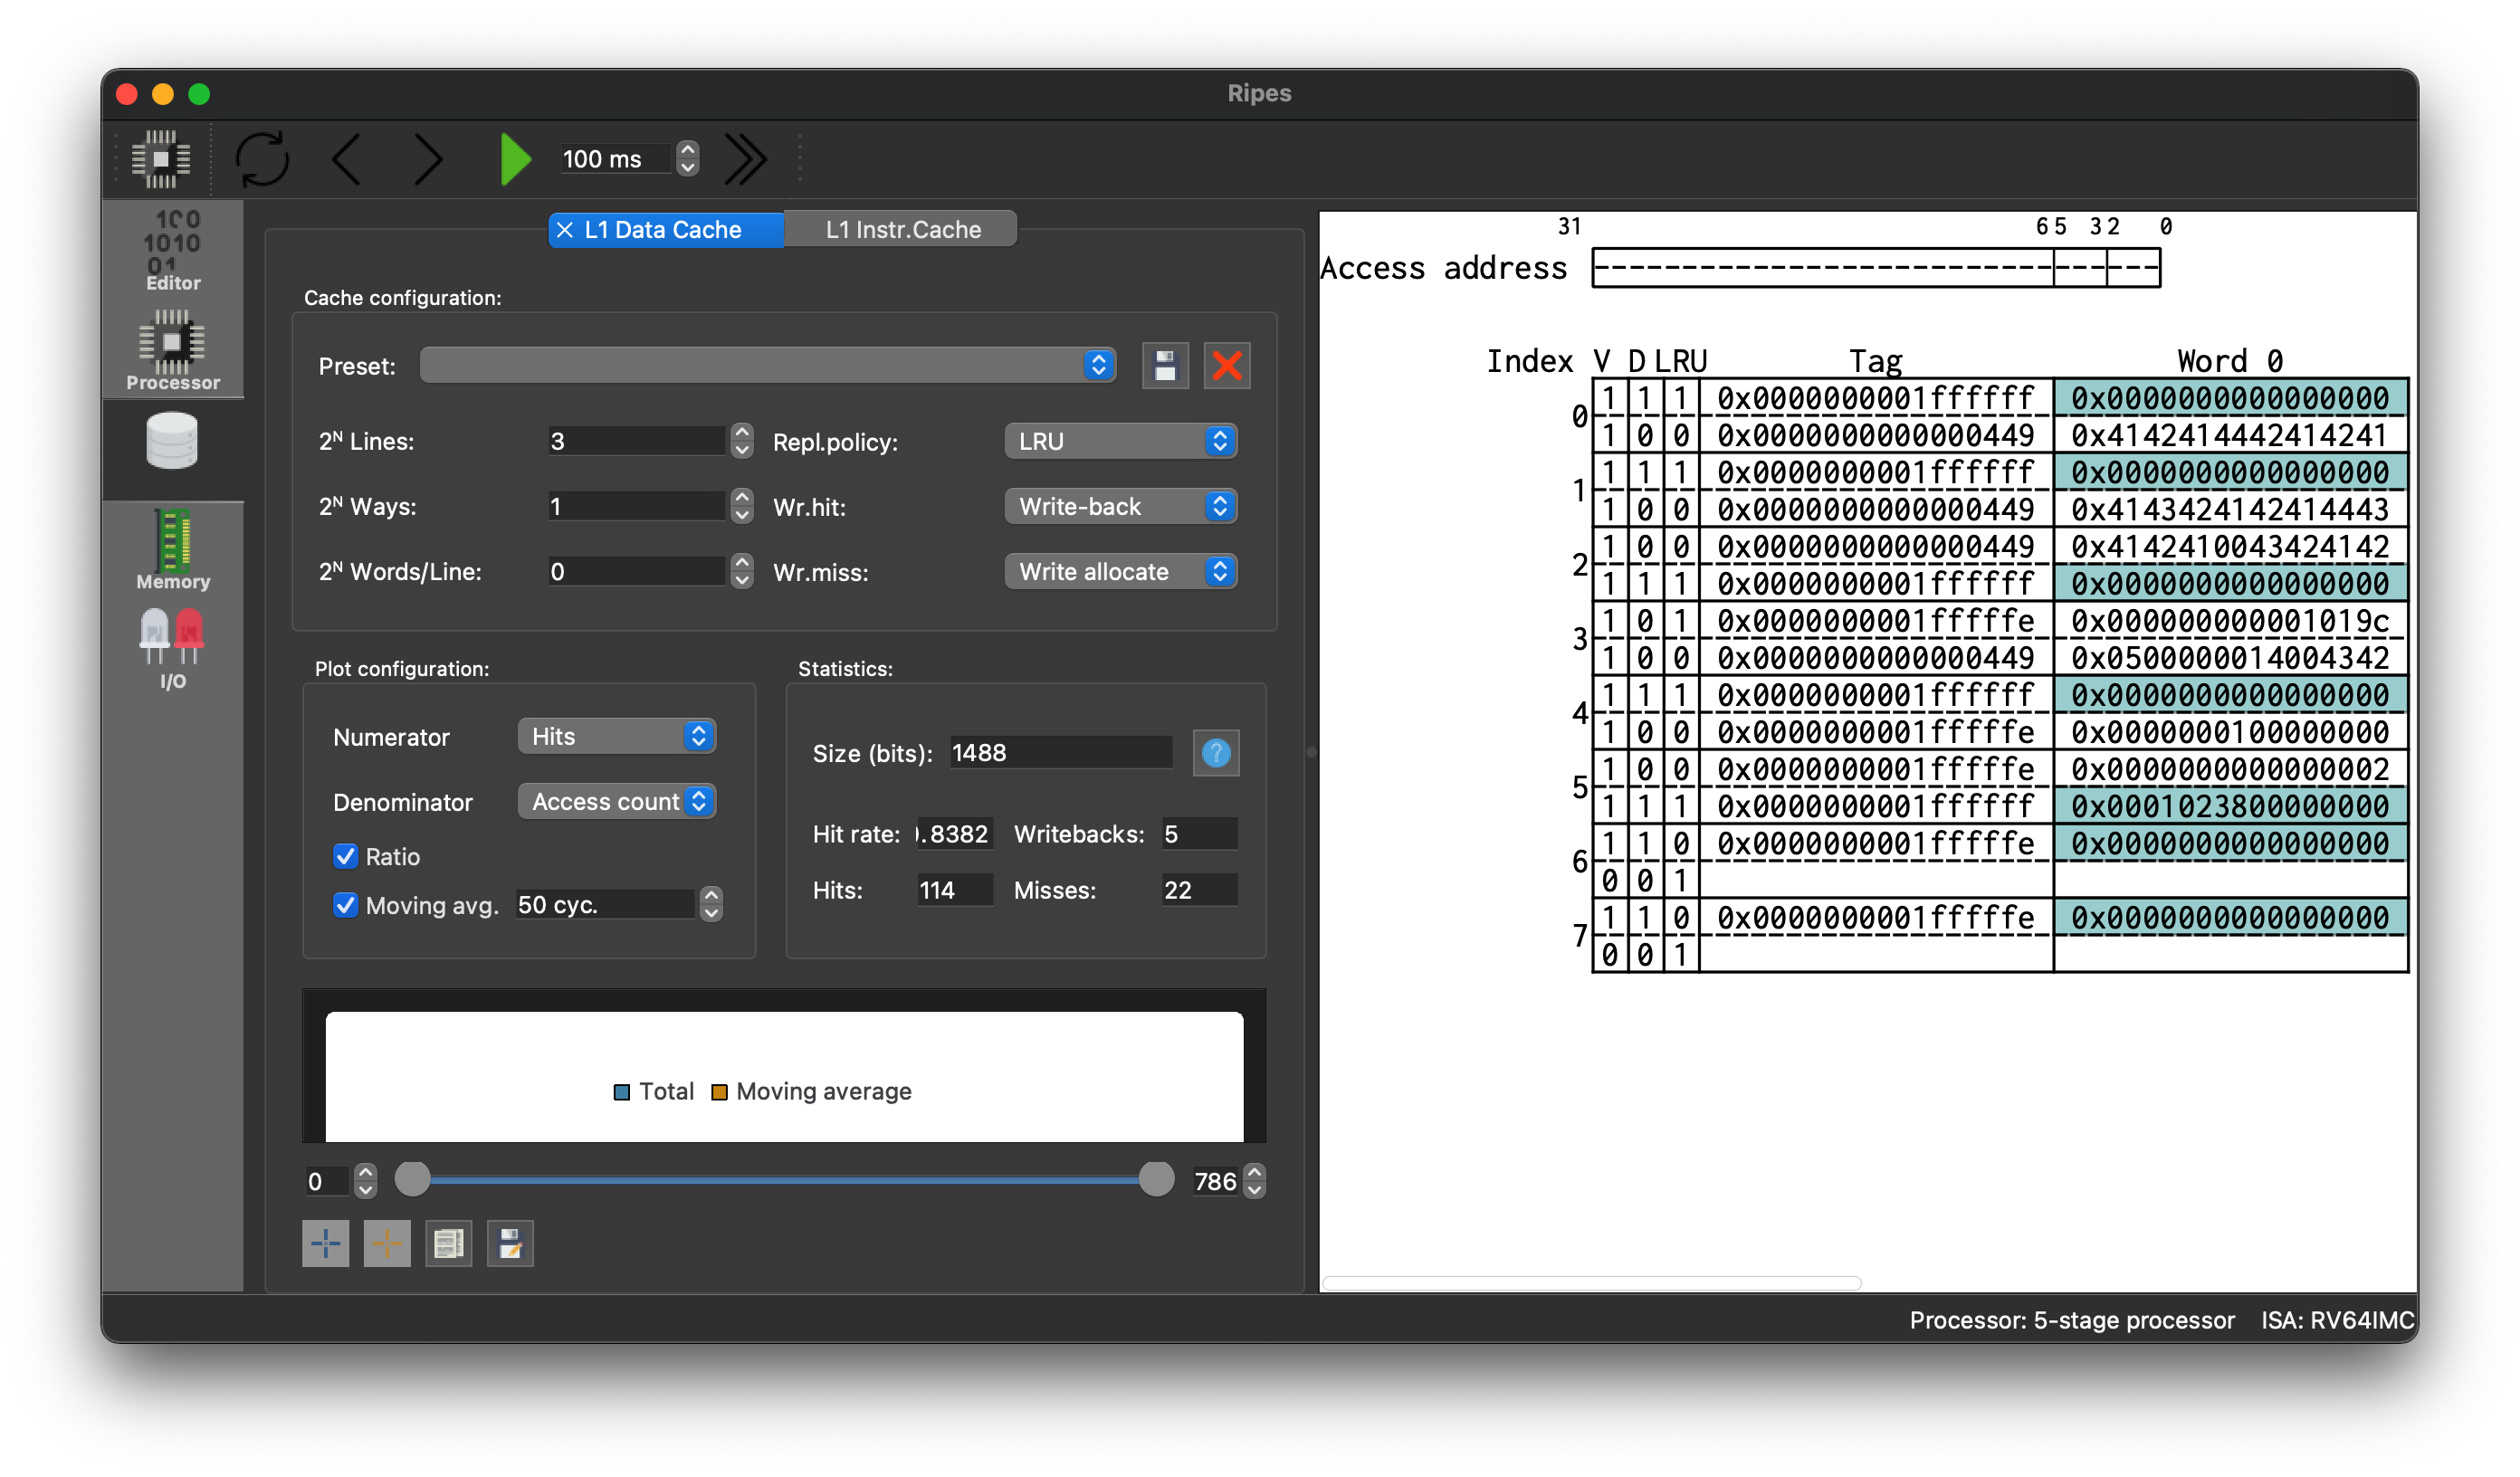
\includegraphics[width=.807\linewidth]{b0}
\caption{Before}
\label{fig:1b0}
\end{subfigure}
\begin{subfigure}{\linewidth}
\centering
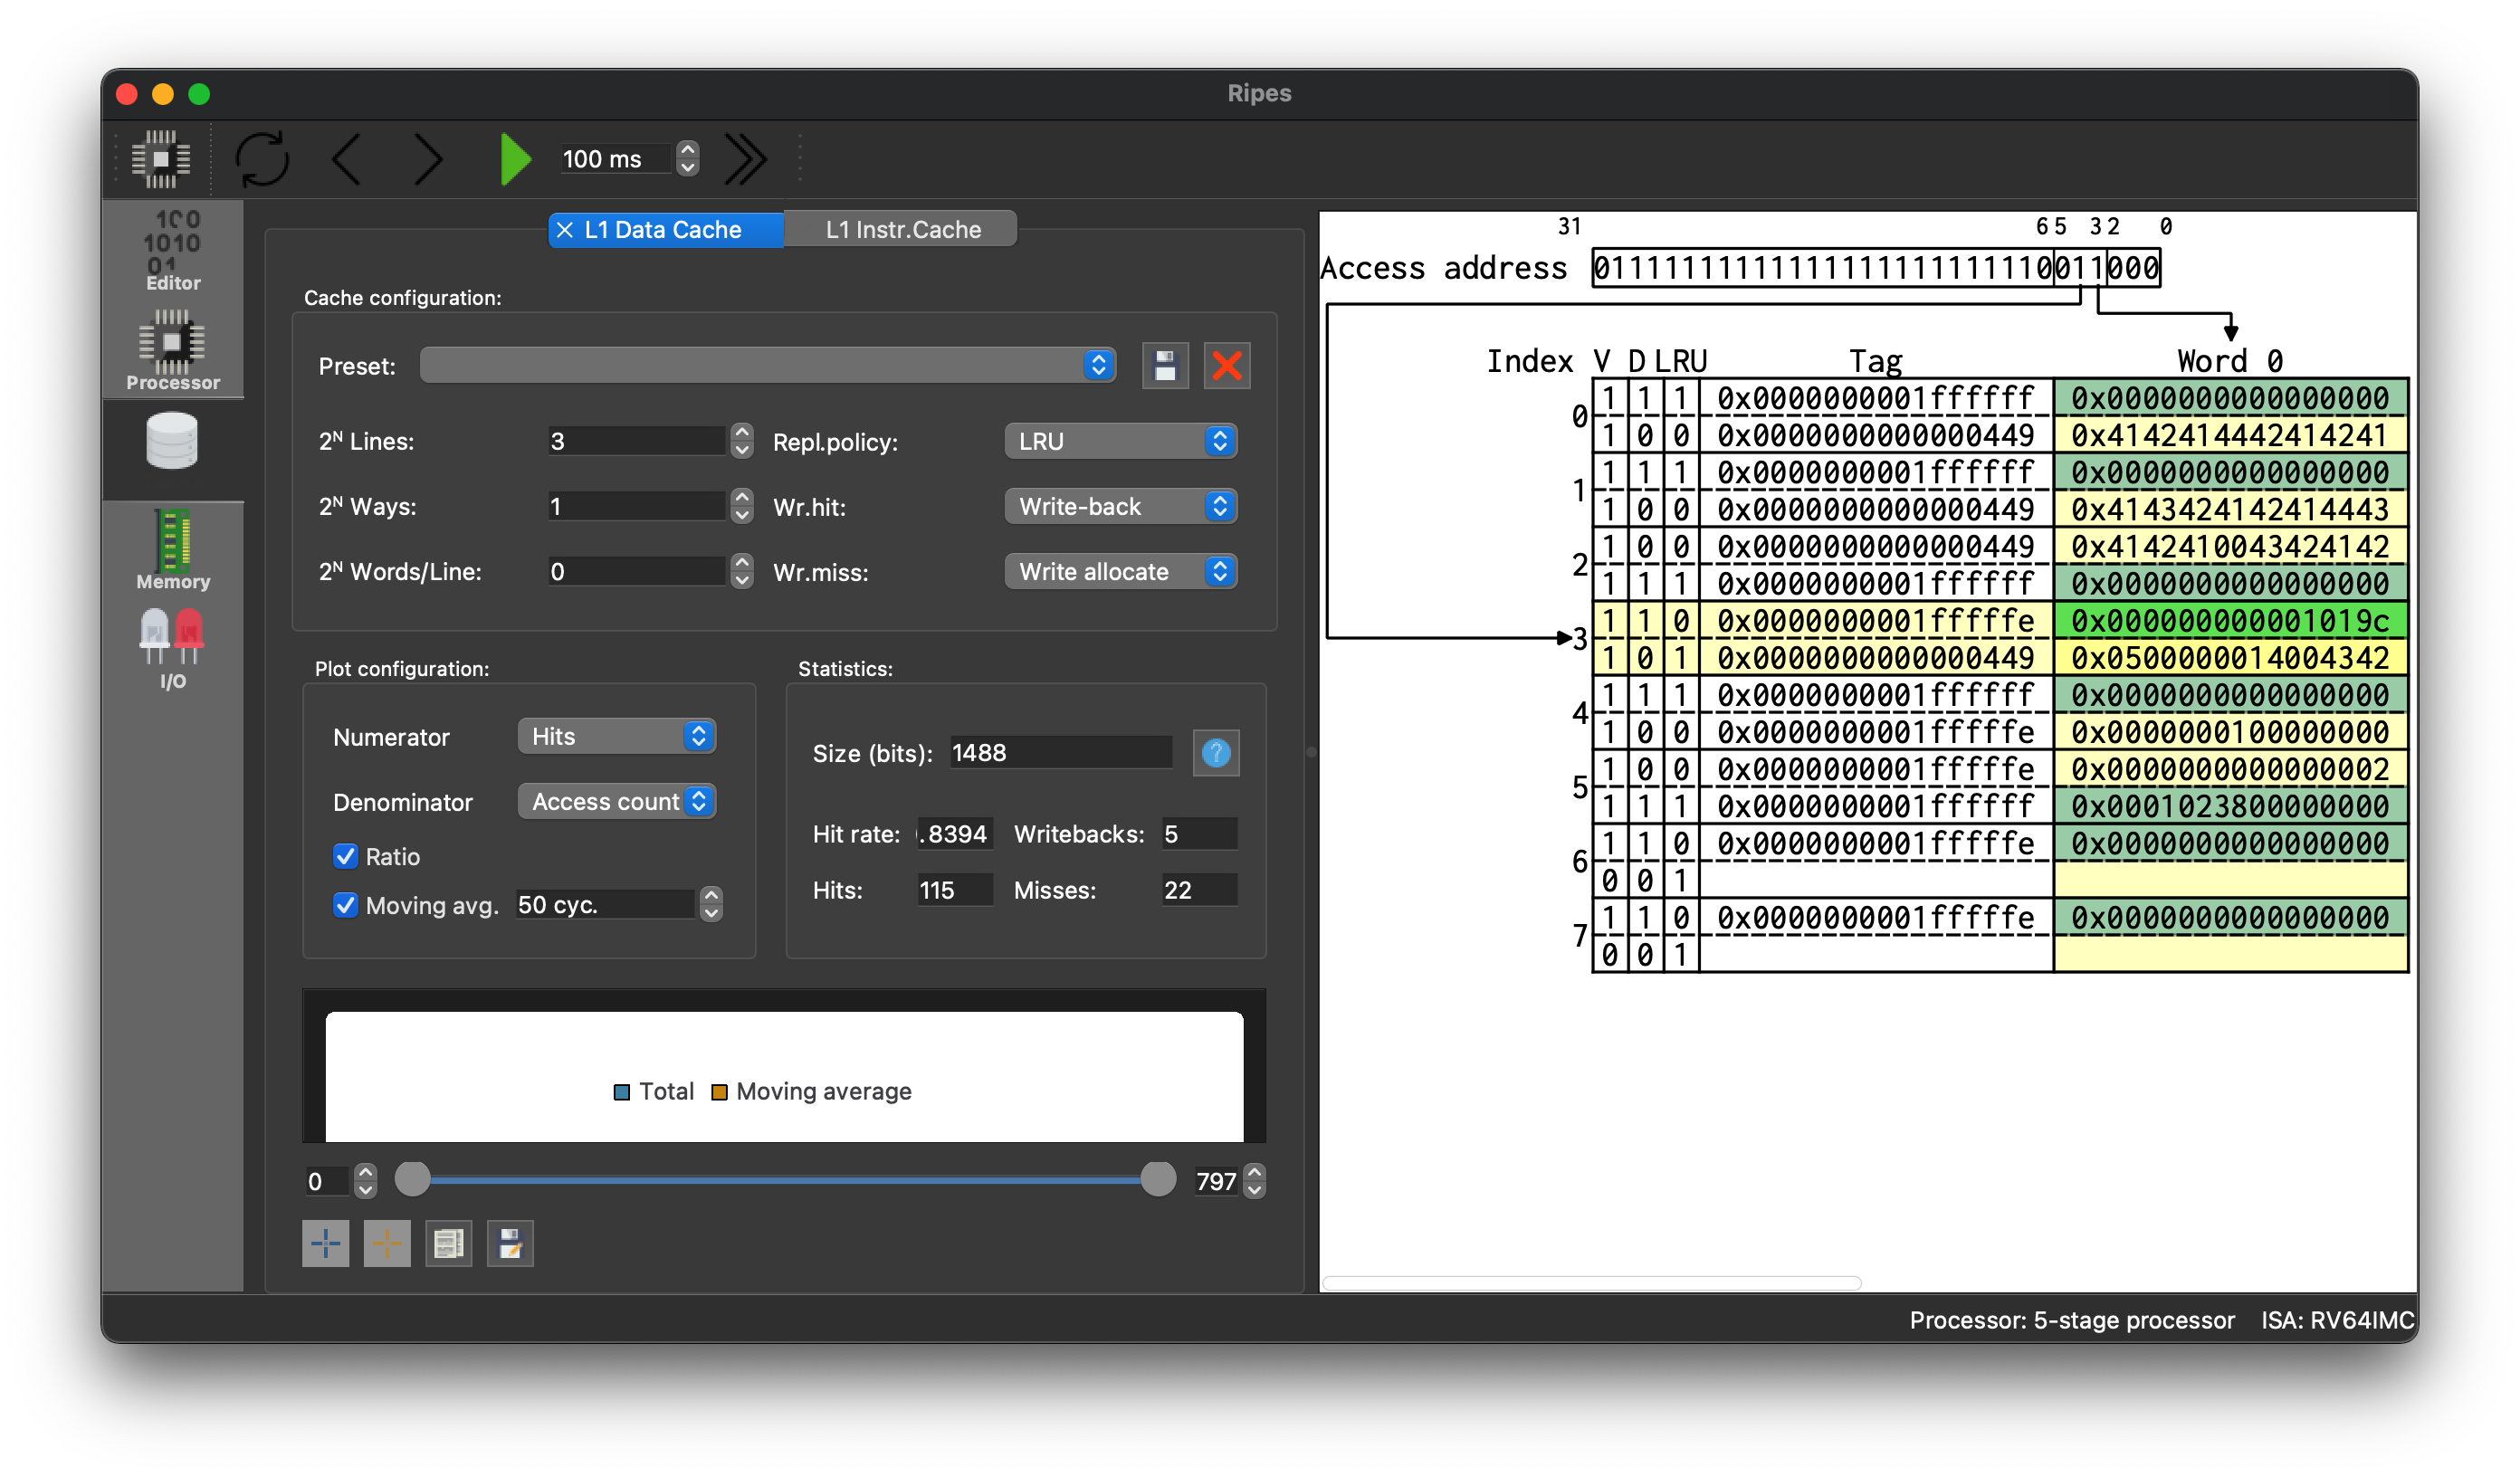
\includegraphics[width=.807\linewidth]{b1}
\caption{After}
\label{fig:1b1}
\end{subfigure}
\caption{Write Hit}
\label{fig:1b}
\end{figure}

The screenshots are in Figure \ref{fig:1b}. Before the \texttt{sw} instruction, the word at address \texttt{0b01111111111111111111111110011000} was fetched in cache already with dirty bit unset. After the write instruction, its dirty bit becomes set thereby.

\subsection{Write Back}

\begin{figure}[htbp]
\begin{subfigure}{\linewidth}
\centering
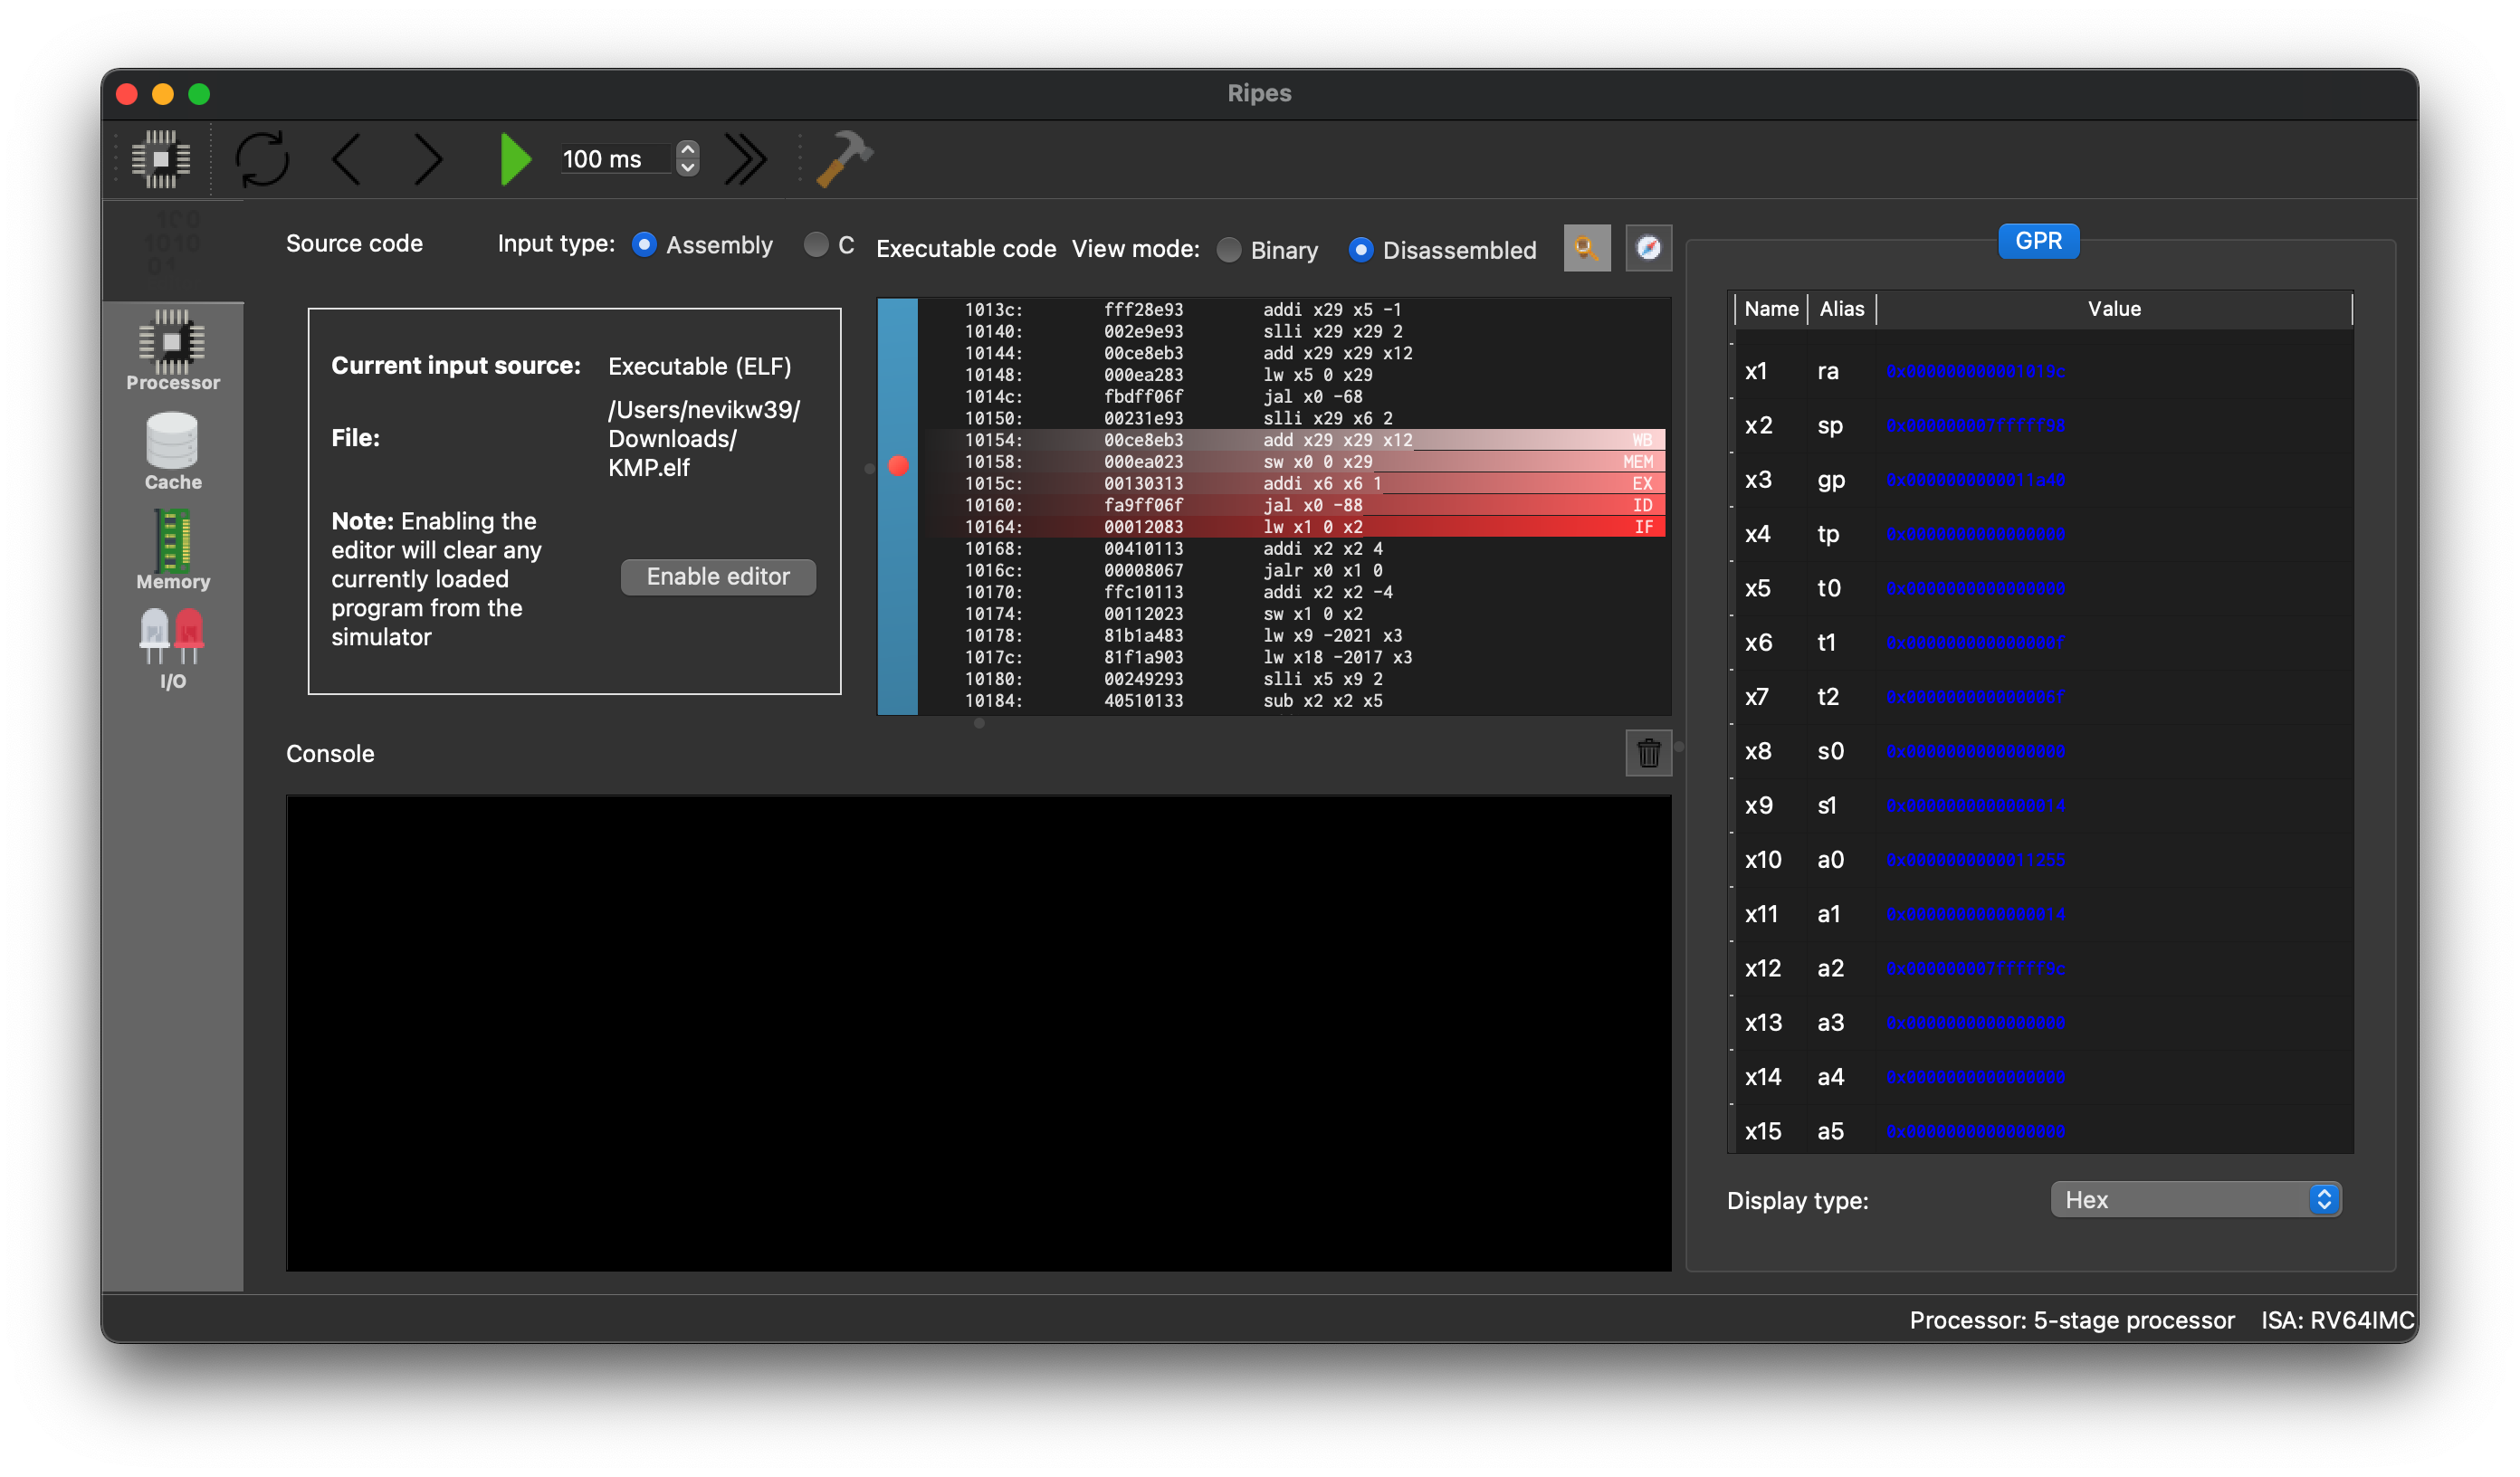
\includegraphics[width=.69\linewidth]{c}
\caption{The instruction}
\end{subfigure}
\begin{subfigure}{\linewidth}
\centering
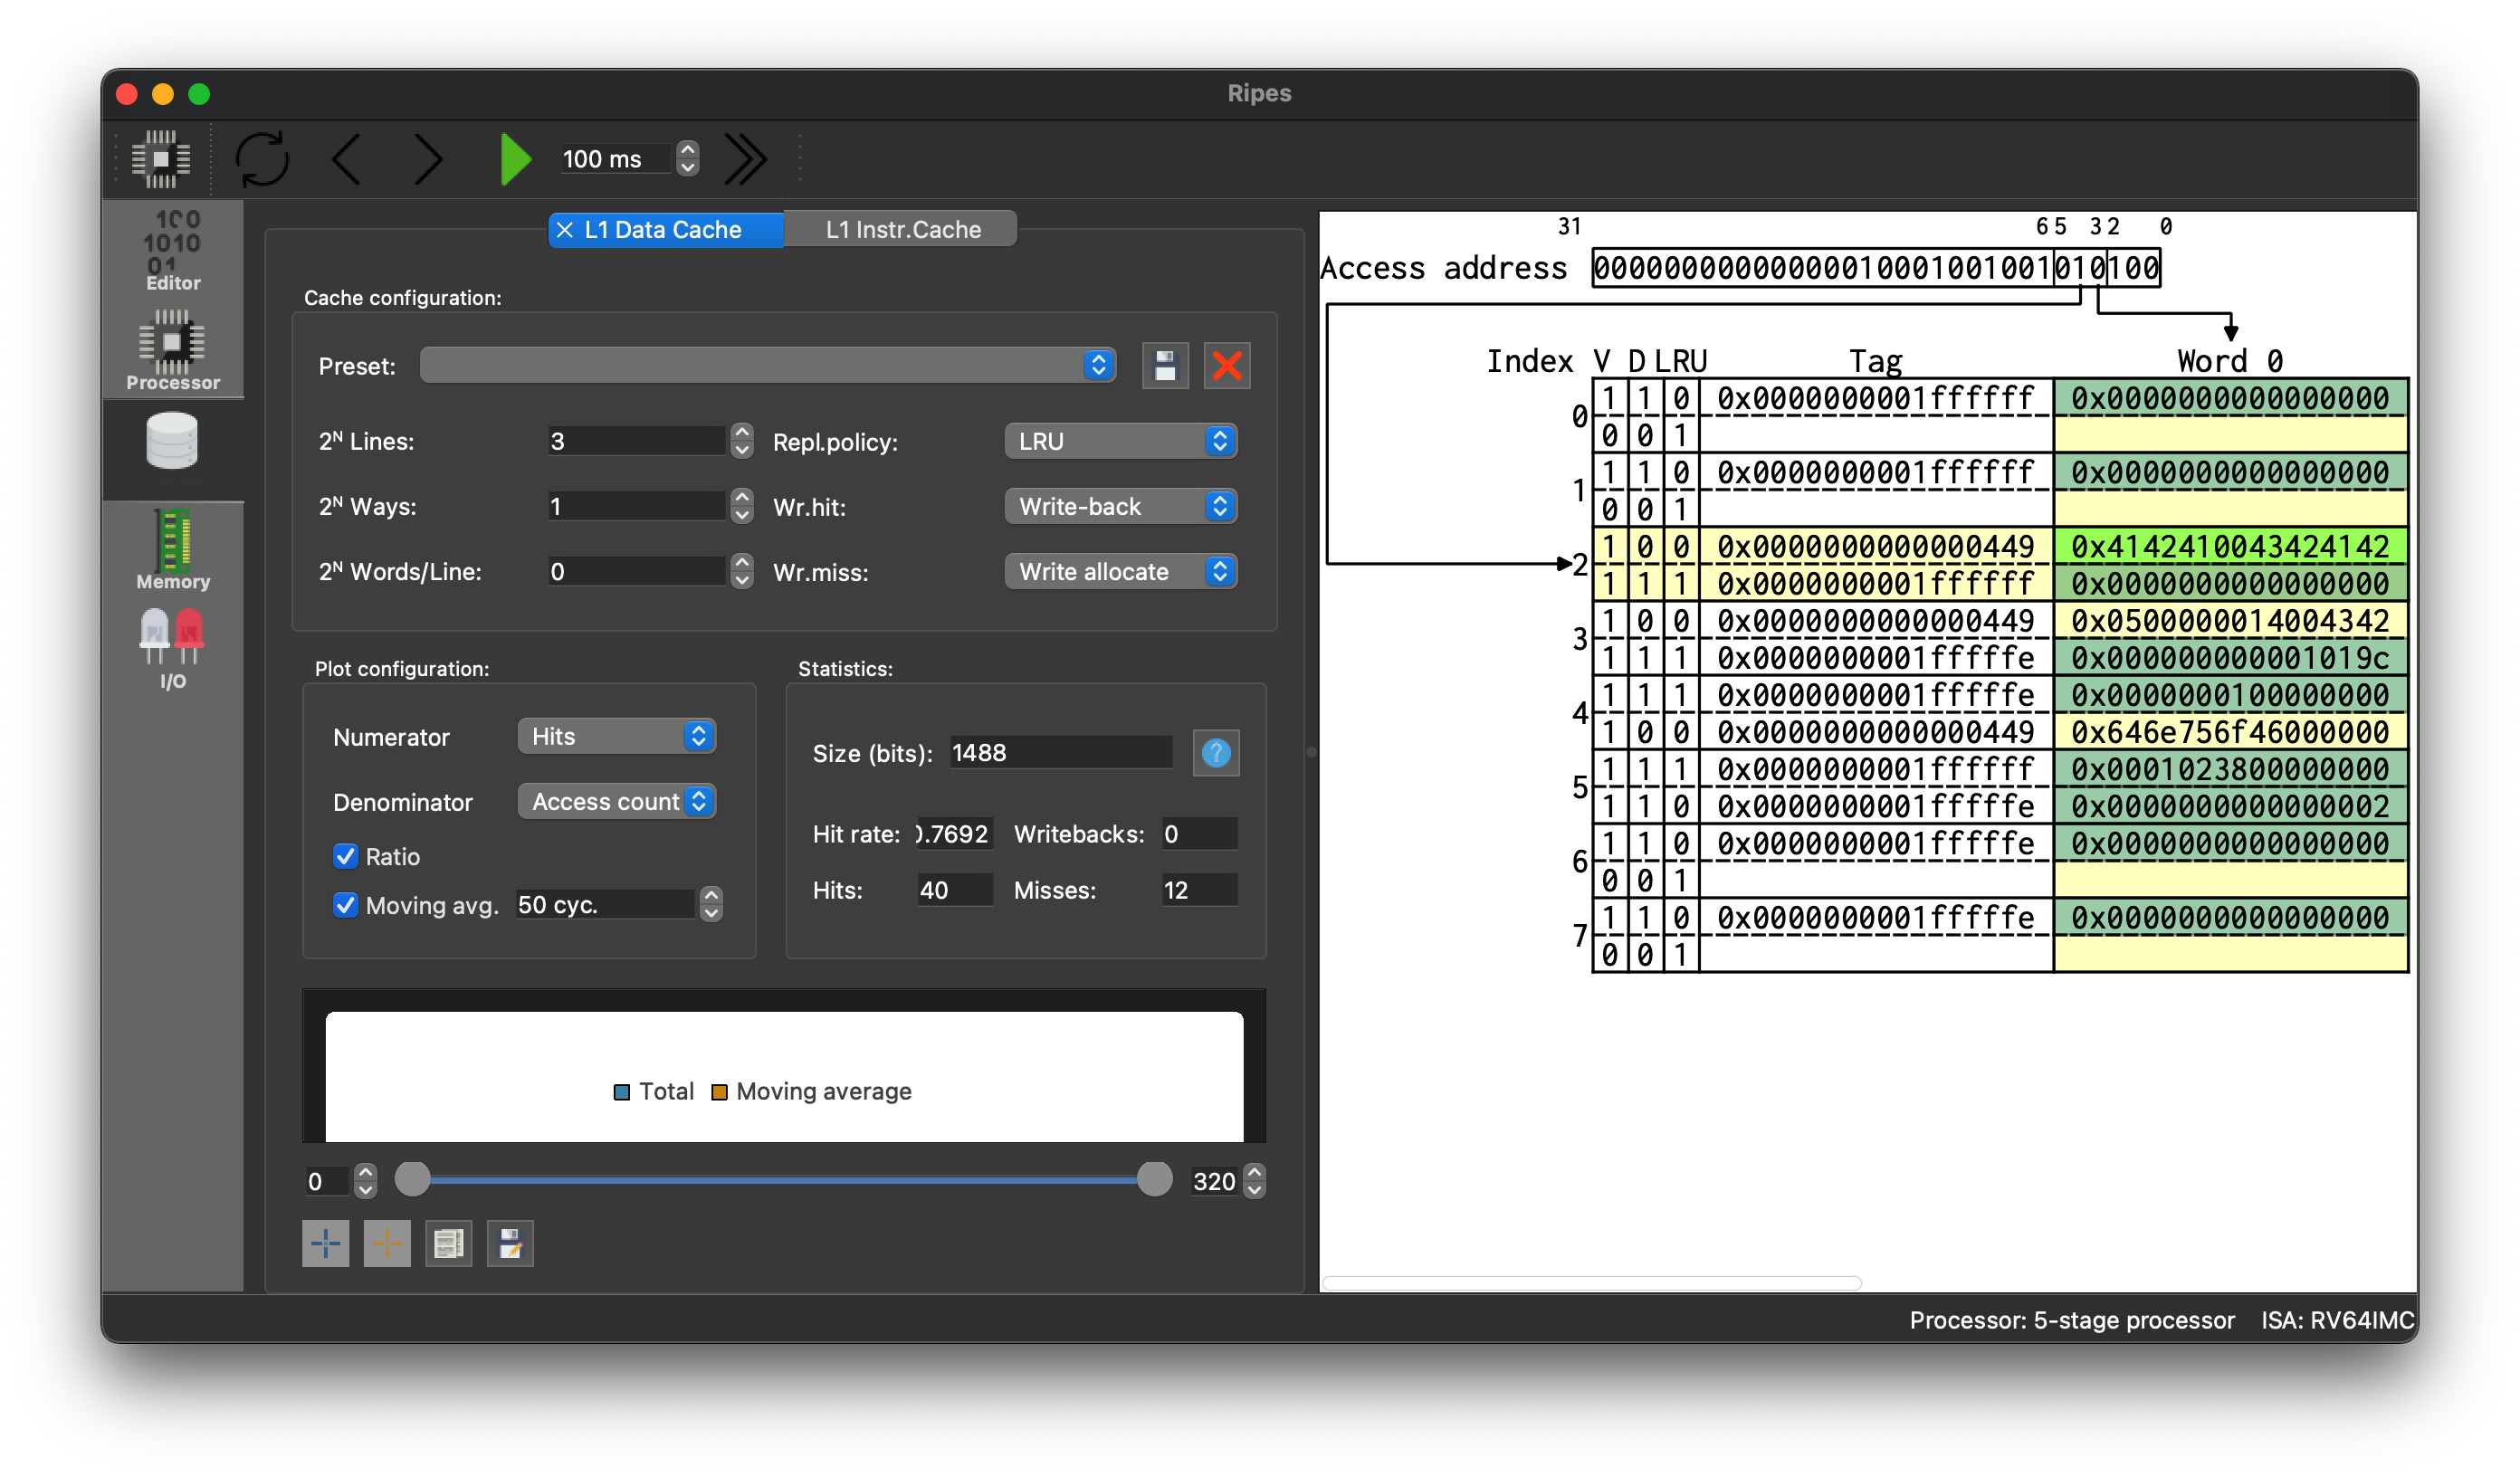
\includegraphics[width=.807\linewidth]{c0}
\caption{Before}
\label{fig:1c0}
\end{subfigure}
\begin{subfigure}{\linewidth}
\centering
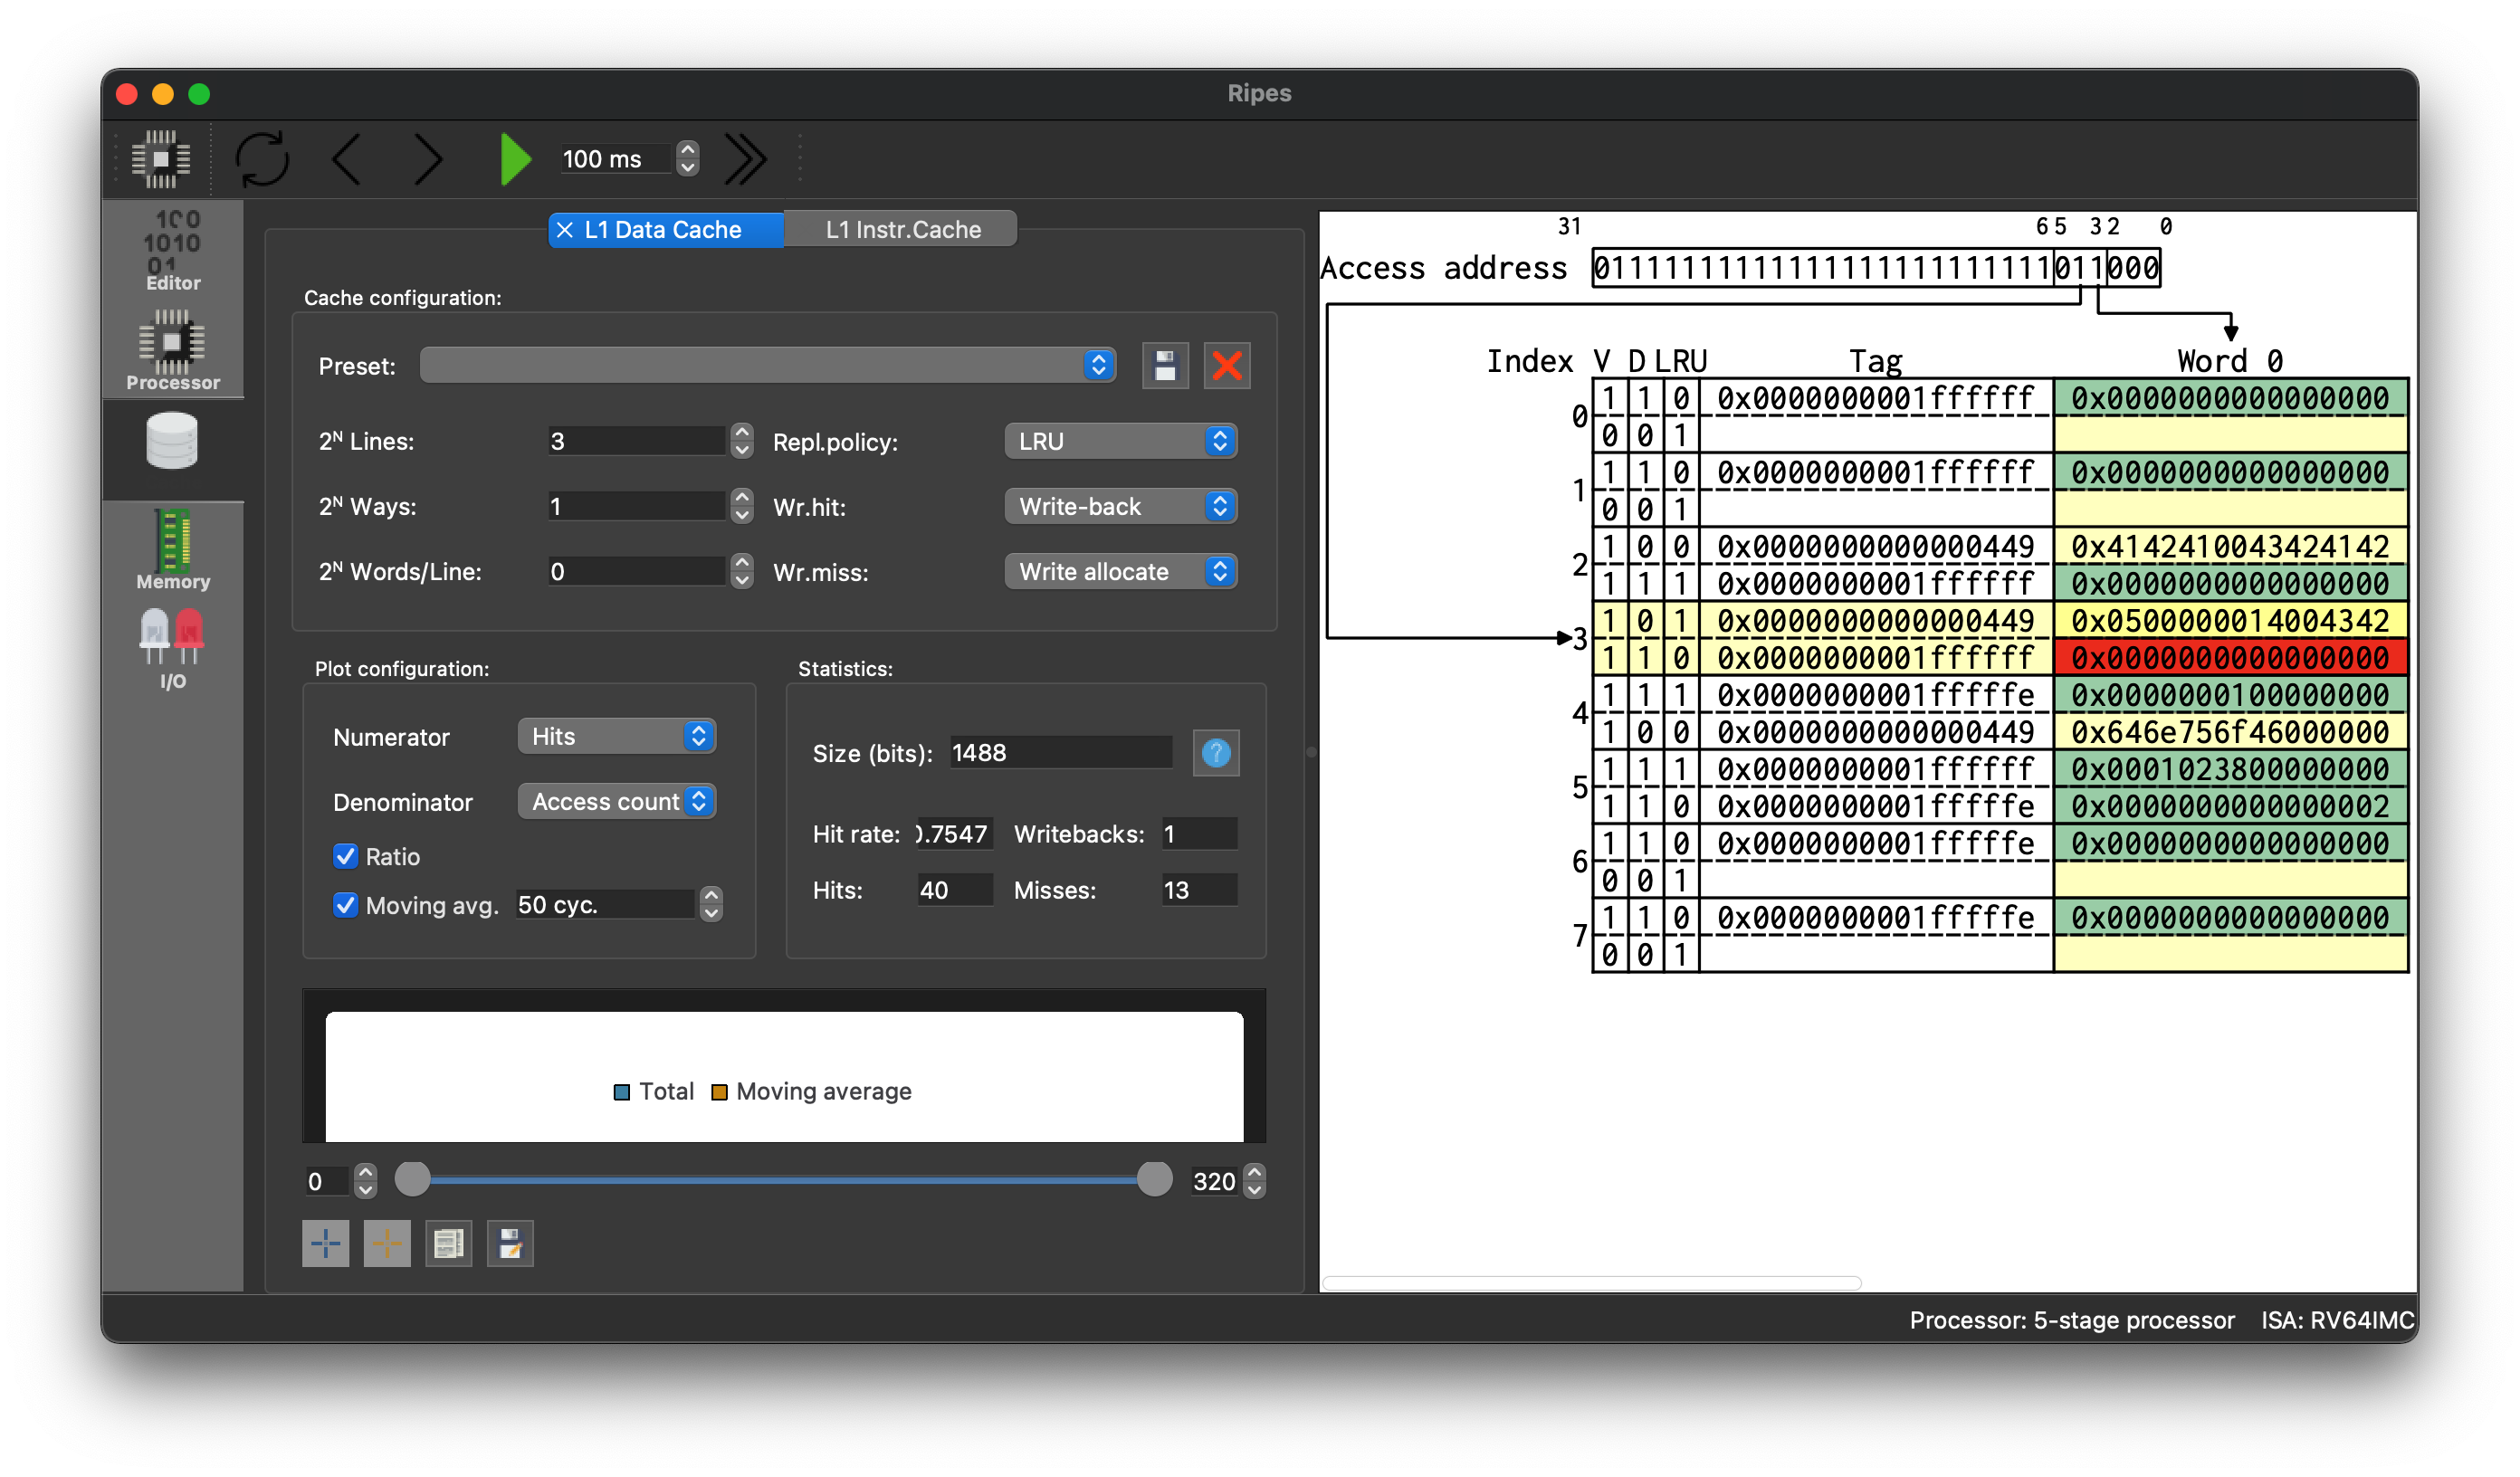
\includegraphics[width=.807\linewidth]{c1}
\caption{After}
\label{fig:1c1}
\end{subfigure}
\caption{Write Back}
\label{fig:1c}
\end{figure}

The screenshots are in Figure \ref{fig:1c}. Before the \texttt{sw} instruction, the set of index 3 was full already and the way whose LRU bit is 1 is dirty. After the instruction conflict to the third set, the dirty way is replaced and written back to upper level of memory.

\pagebreak

\section{Cache Improvement}

The original hit rate was $0.8606$. Taking the same size of 16 words, I decide to have 4 words per block and increase the number of ways to $2^2=4$, which is equivalent to fully associative. As a consequence, the spatial and temporal localities are well utilized and the hit rate becomes $0.9455$.

\begin{figure}[htbp]
\begin{subfigure}{\linewidth}
\centering
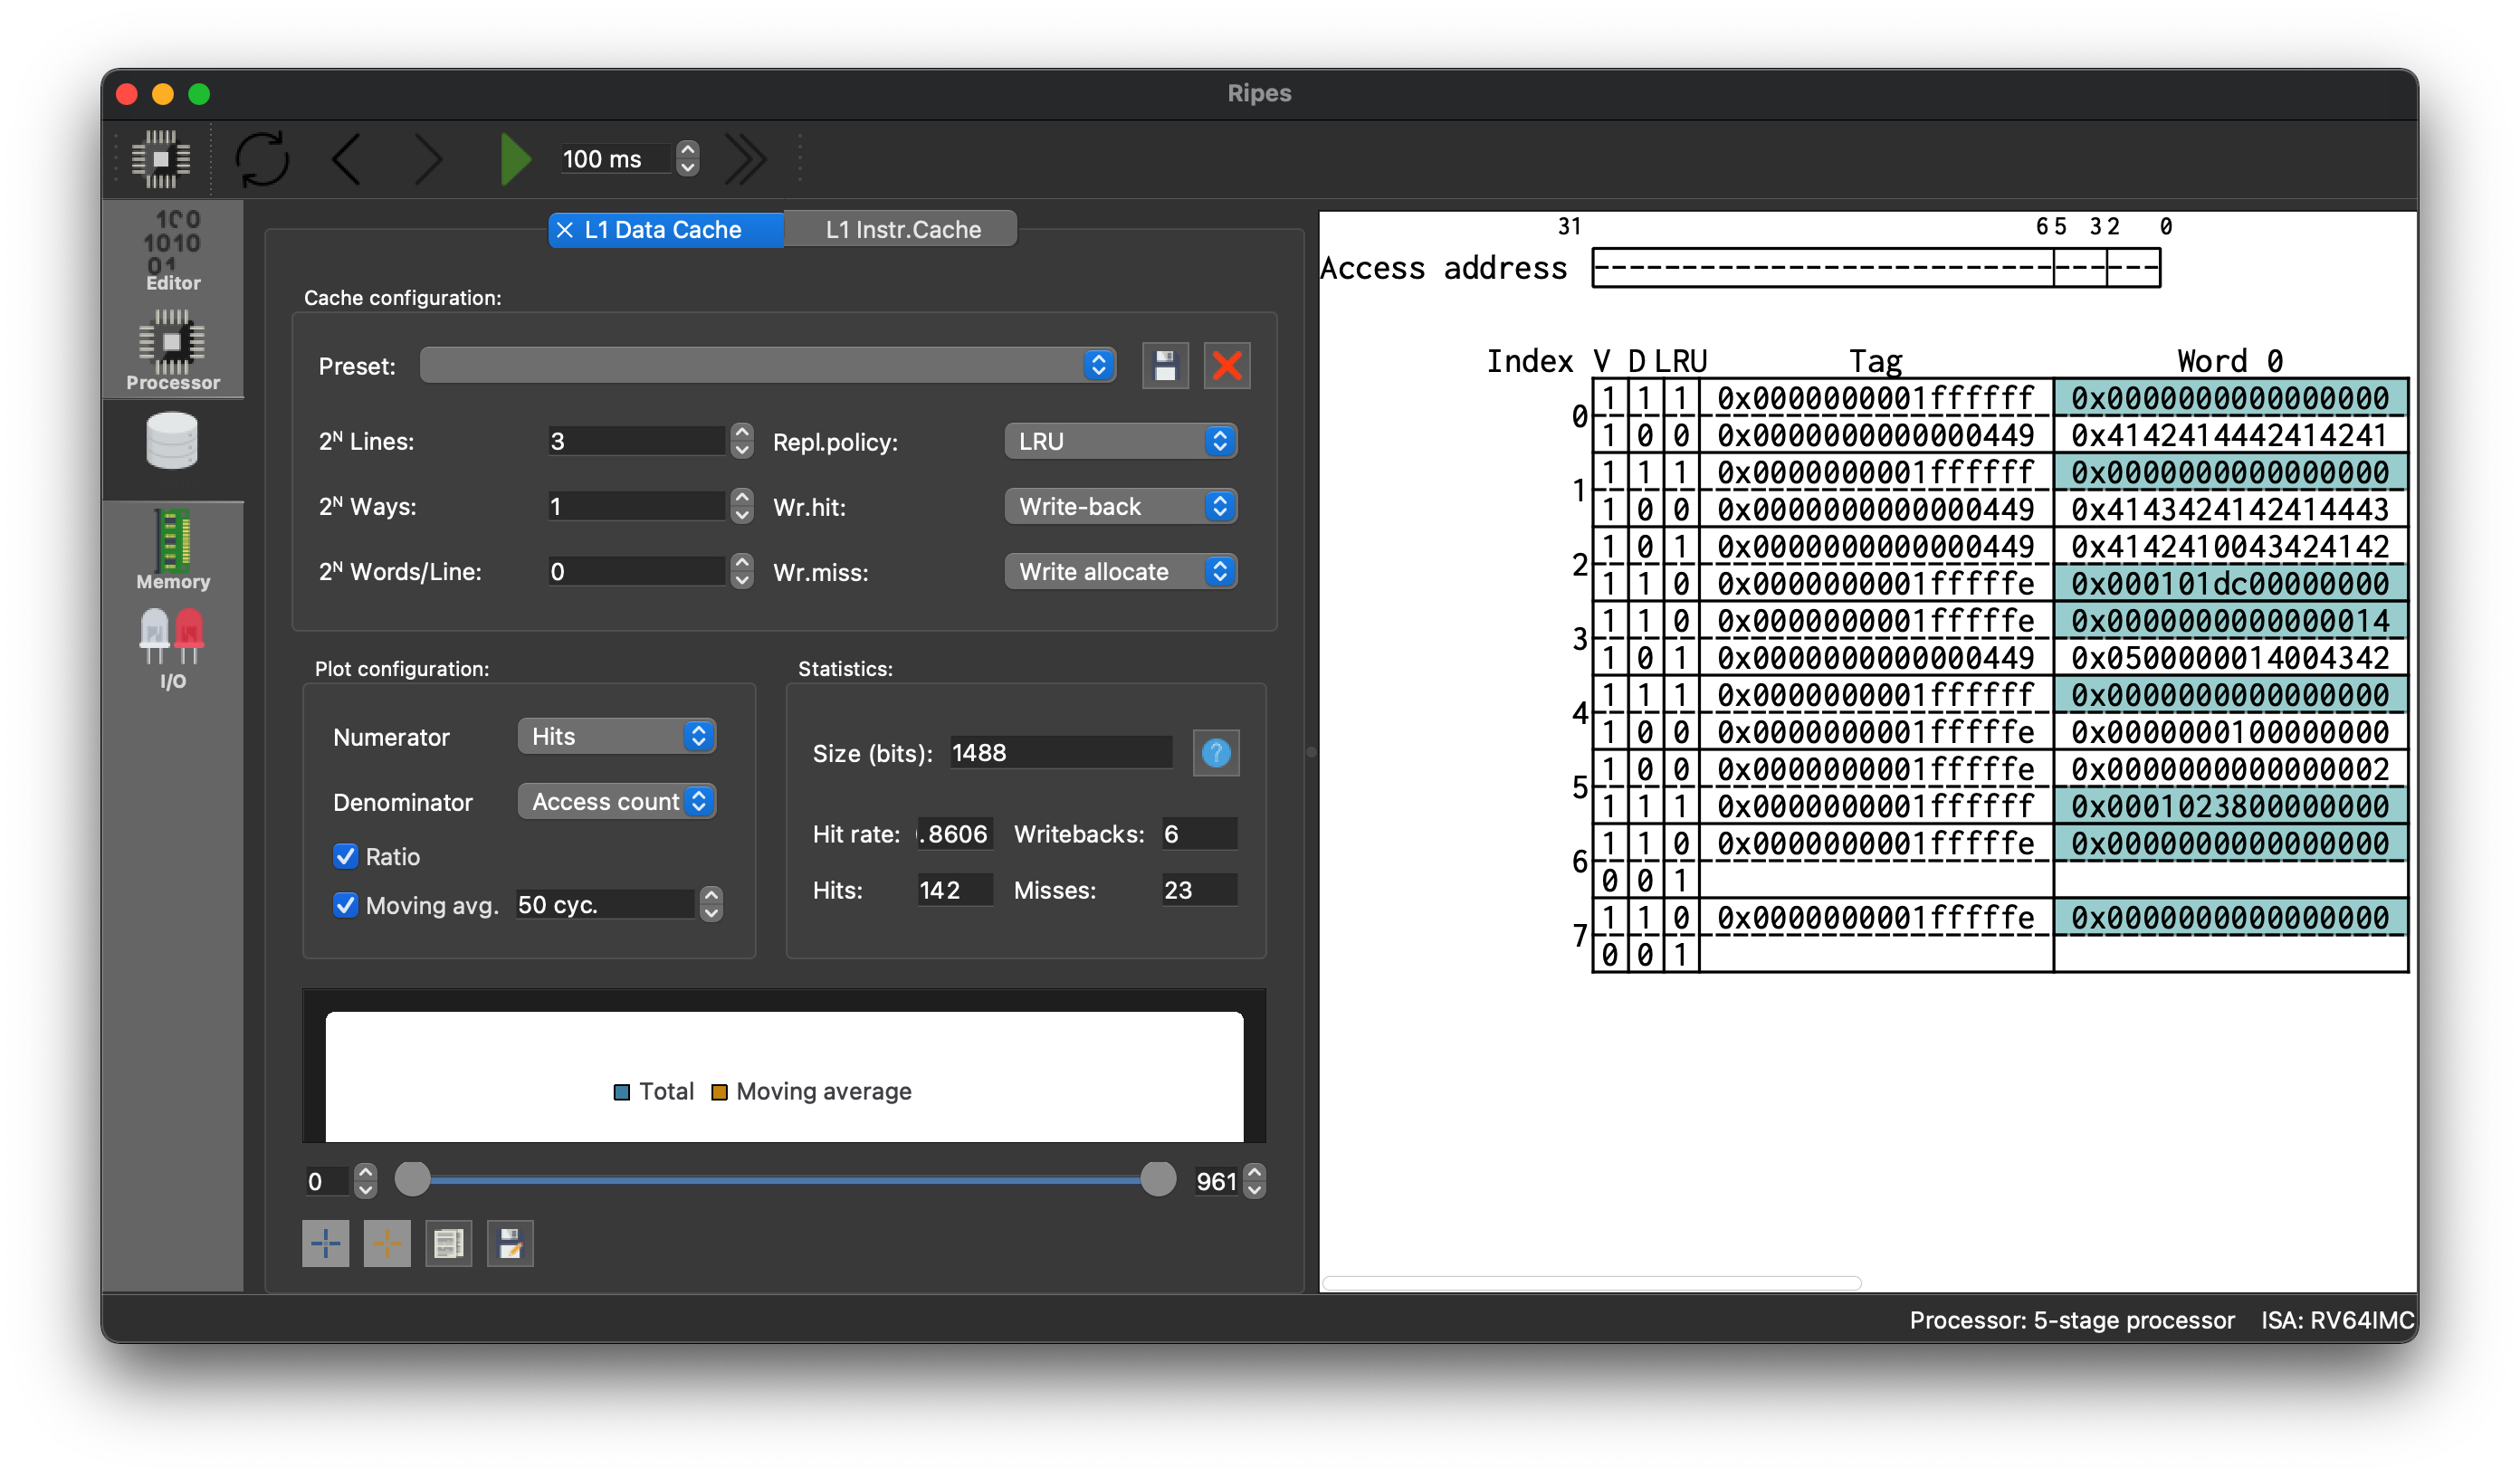
\includegraphics[width=.8597\linewidth]{2-way}
\caption{Orignal}
\label{fig:2a}
\end{subfigure}
\begin{subfigure}{\linewidth}
\centering
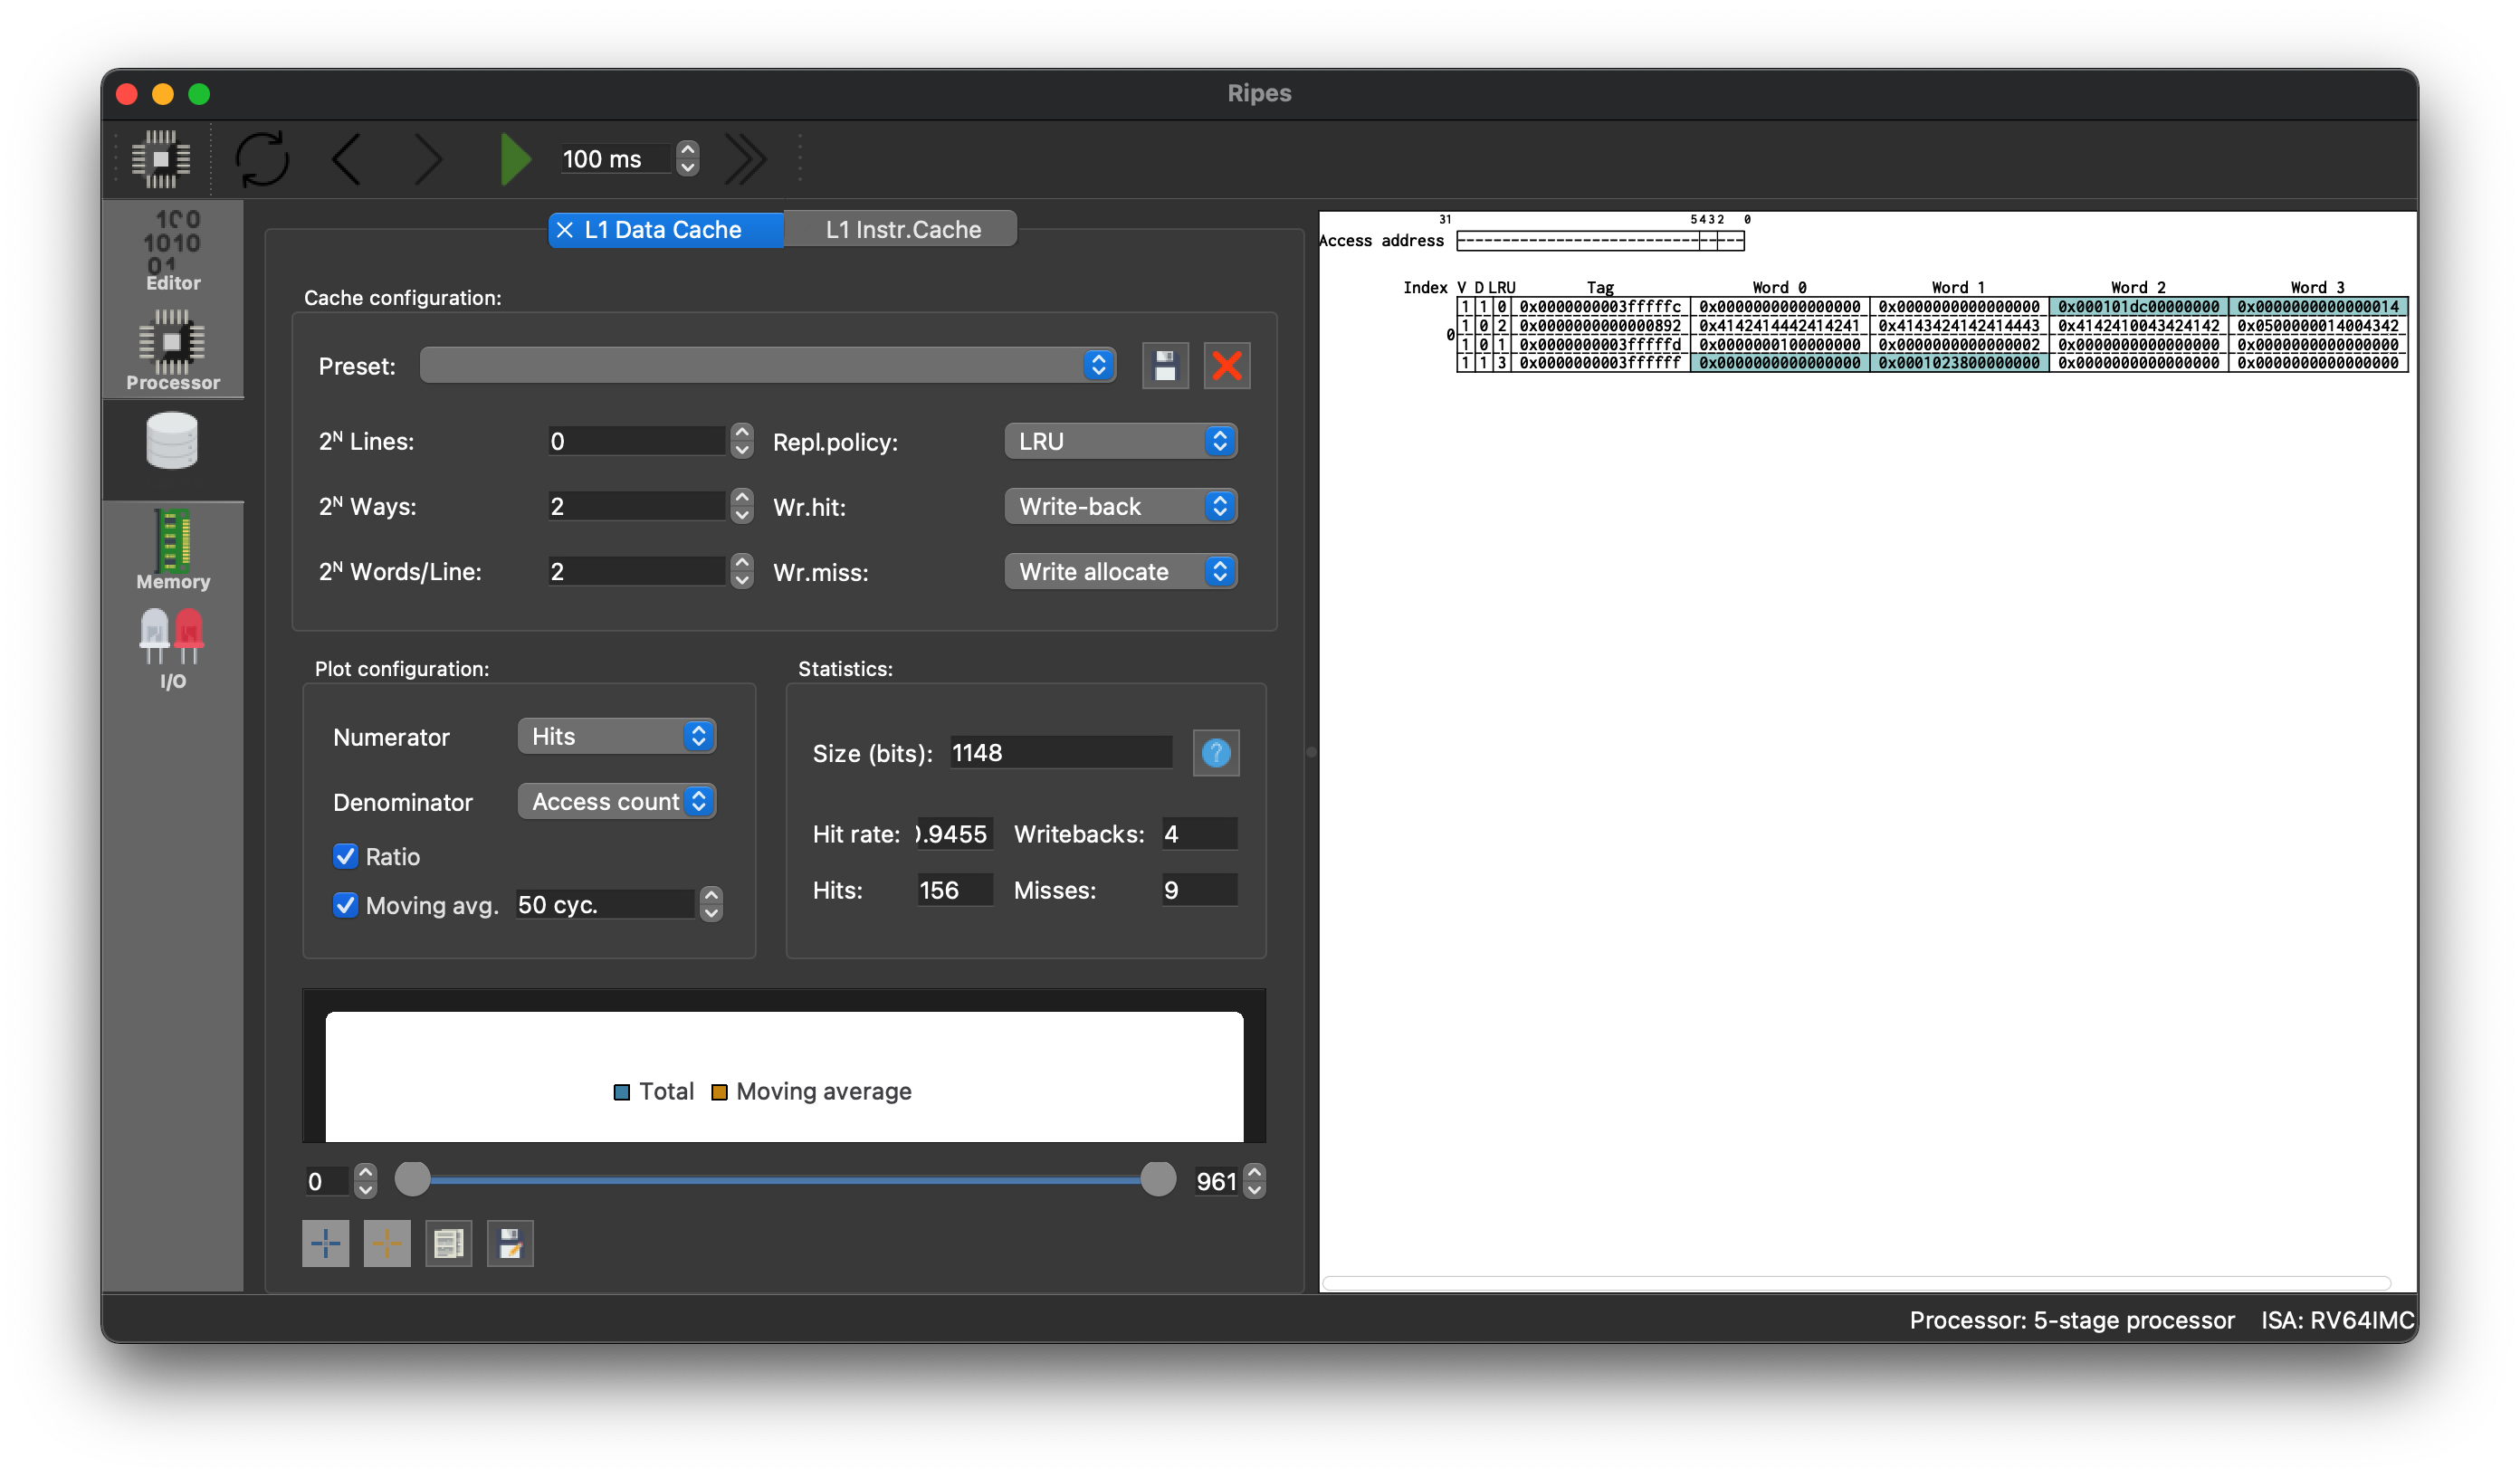
\includegraphics[width=.8597\linewidth]{fully}
\caption{Improvement}
\label{fig:2b}
\end{subfigure}
\caption{Cache Improvement}
\label{fig:2}
\end{figure}

\section{Cache Configurations}

\subsection{Sizes}

Assume that the machine is word-addressable and addresses are to words.

\begin{table}[hbp]
\caption{Cache Sizes}
\label{tab:cache_size}
\centering
\begin{tabular}{ccccc}
\# & Tag & Index & Offset & Total size \\
\hline
1 & $20-\lg16-\lg1=16$ & $\lg16=4$ & $\lg1=0$ & 784 \\
2 & $20-\lg\frac{16}{4}-\lg4=16$ & $\lg\frac{16}{4}=2$ & $\lg4=2$ & 580 \\
3 & $20-\lg16\frac{16}{2\times2}-\lg2=17$ & $\lg\frac{16}{2\times2}=2$ & $\lg2=1$ & 656 \\
4 & $20-\lg4=18$ & 0 & $\lg4=2$ & 588
\end{tabular}
\end{table}

The number of bits of total size is $(1+\#\text{BITS}(\text{tag}))\times\frac{16}{\text{words per block}}+16\times32$.

\subsection{Example}

\subsubsection{Accesses}

\begin{table}[hbp]
\caption{Access Results}
\label{tab:cache_access}
\centering
\begin{tabular}{cccc}
Address & \#2 & \#3 & \#4 \\
\hline
16 & Compulsory miss & Compulsory miss & Compulsory miss \\
17 & Hit!! & Hit!! & Hit!! \\
18 & Hit!! & Compulsory miss & Hit!! \\
19 & Hit!! & Hit!! & Hit!! \\
20 & Compulsory miss & Compulsory miss & Compulsory miss \\
48 & Compulsory miss & Compulsory miss & Compulsory miss \\
49 & Hit!! & Hit!! & Hit!! \\
17 & Conflict miss & Hit!! & Hit!! \\
48 & Conflict miss & Hit!! & Hit!! \\
49 & Hit!! & Hit!! & Hit!! \\
17 & Conflict miss & Hit!! & Hit!! \\
5 & Compulsory miss & Compulsory miss & Compulsory miss \\
6 & Hit!! & Hit!! & Hit!! \\
7 & Hit!! & Compulsory miss & Hit!!
\end{tabular}
\end{table}

\subsubsection{Final Contents}

\begin{table}[hbp]
\caption{Cache \#2}
\label{tab:cache_content2}
\centering
\begin{tabular}{crrc}
Index & Valid & Tag & Data \\
\hline
00 & 1 & 1 & words of memory address 16, 17, 18, 19 \\
01 & 1 & 0 & words of memory address 4, 5, 6, 7 \\
10 & 0 \\
11 & 0
\end{tabular}
\end{table}

\begin{table}[hbp]
\caption{Cache \#3}
\label{tab:cache_content3}
\centering
\begin{tabular}{crrc}
Set & Valid & Tag & Data \\
\hline
00 & 1 & 10 & words of memory address 16, 17 \\
00 & 1 & 110 & words of memory address 48, 49 \\
01 & 1 & 10 & words of memory address 18, 19 \\
01 & 0 \\
10 & 1 & 1 & words of memory address 20, 21 \\
10 & 1 & 0 & words of memory address 4, 5 \\
11 & 1 & 0 & words of memory address 6, 7 \\
11 & 0
\end{tabular}
\end{table}

\section{Hamming Codes}

\subsection{Single Error Correction}

$$
\left\{\begin{array}{l}
h_1=1\oplus0\oplus1\oplus0=0\\
h_2=1\oplus0\oplus0\oplus0=1\\
h_4=1\oplus1\oplus0\oplus0=0
\end{array}\right.
$$, so we have $H=\{0,1,0\}=2$, indicating that the second bit, $p2$, is an error.

\subsection{Single Error Correction \& Double Error Detection}

$$
\left\{\begin{array}{l}
h_1=1\oplus1\oplus0\oplus0=0\\
h_2=0\oplus1\oplus1\oplus0=0\\
h_4=1\oplus0\oplus1\oplus0=0\\
h_8=1\oplus0\oplus1\oplus1\oplus0\oplus1\oplus0\oplus1=1
\end{array}\right.
$$, so we have $H=0$ and $p_8=1$, indicating that the last bit, $p_8$, is an error.

\subsection{Yet Another Single Error Correction \& Double Error Detection}

$$
\left\{\begin{array}{l}
h_1=1\oplus0\oplus1\oplus1=1\\
h_2=0\oplus0\oplus0\oplus1=1\\
h_4=0\oplus1\oplus0\oplus1=0\\
h_8=1\oplus0\oplus0\oplus0\oplus1\oplus0\oplus1\oplus1=0
\end{array}\right.
$$, so we have $H=\{0,1,1\}=3$ but $h_8=0$, indicating that the double error occurred.

\section{Cache Performance}

\subsection{Miss Penalties \& Memory Stall Cycles}

\begin{table}[hbp]
\caption{}
\label{tab:miss_penalty_mem_stall_cyc}
\centering
\begin{tabular}{c|cc}
\# & 1 & 2 \\
Miss Penalty & $5+4=9$ & $5+2=7$ \\
Mem. Stall Cyc. & $70000\times(4\%+\frac{1}{3}\times3\%)\times9=31500$ & $70000\times(4\%+\frac{1}{3}\times3\%)\times7=24500$
\end{tabular}
\end{table}

\subsection{Effective CPI}

$$\text{Base CPI}=1.7-(4\%+\frac{1}{3}\times3\%)\times(5+1)=1.4$$

\begin{table}[hbp]
\caption{}
\label{tab:cpi}
\centering
\begin{tabular}{c|cc}
\# & 1 & 2 \\
CPI & $1.4+(4\%+\frac{1}{3}\times3\%)\times(5+4)=1.85$ & $1.4+(4\%+\frac{1}{3}\times3\%)\times(5+2)=1.75$
\end{tabular}
\end{table}

\section{Virtual Memory}

$$\#\text{blocks in cache}=\frac{64\times1024}{256}=256$$

\begin{table}[hbp]
\caption{}
\label{tab:virt}
\centering
\begin{tabular}{cccc}
Virtual address & Physical address & Cache & TLB \\
\hline
\texttt{0x954a16c2} & \texttt{0x3b9416c2} & Miss & Miss \\
\texttt{0x6542c746} & \texttt{0x0ae6c746} & Miss & Miss \\
\texttt{0x954a1647} & \texttt{0x3b941647} & Hit!! & Hit!! \\
\texttt{0x6542c412} & \texttt{0x0ae6c412} & Miss & Hit!! \\
\texttt{0x2b74c4d3} & \texttt{0x14acc4d3} & Miss & Miss \\
\texttt{0x6542c46a} & \texttt{0x0ae6c46a} & Miss & Hit!! \\
\texttt{0x954a16dd} & \texttt{0x3b9416dd} & Hit!! & Miss \\
\texttt{0x6542c417} & \texttt{0x0ae6c417} & Hit!! & Hit!! \\
\texttt{0x2b74c723} & \texttt{0x14acc723} & Miss & Miss \\
\end{tabular}
\end{table}

\end{document}
